\documentclass[9pt]{beamer}

% Beamer style
%\usetheme[secheader]{Madrid}
% \usetheme{CambridgeUS}
\useoutertheme{infolines}
\usecolortheme[rgb={0.65,0.15,0.25}]{structure}
% \usefonttheme[onlymath]{serif}
\beamertemplatenavigationsymbolsempty
%\AtBeginSubsection

% Packages
%\usepackage[french]{babel}
\usepackage[latin1]{inputenc}
\usepackage{color}
% \usepackage[dvipsnames]{xcolor}
\usepackage{xspace}
\usepackage{dsfont, stmaryrd}
\usepackage{amsmath, amsfonts, amssymb, stmaryrd, mathabx}
\usepackage{epsfig}
\usepackage{multirow}
\usepackage{tikz}
\usepackage{url}
% \usepackage{ulem}
\usepackage{/home/robin/LATEX/Biblio/astats}
%\usepackage[all]{xy}
\usepackage{graphicx}

% Maths
% \newtheorem{theorem}{Theorem}
% \newtheorem{definition}{Definition}
\newtheorem{proposition}{Proposition}
% \newtheorem{assumption}{Assumption}
% \newtheorem{algorithm}{Algorithm}
% \newtheorem{lemma}{Lemma}
% \newtheorem{remark}{Remark}
% \newtheorem{exercise}{Exercise}
% \newcommand{\propname}{Prop.}
% \newcommand{\proof}{\noindent{\sl Proof:}\quad}
% \newcommand{\eproof}{$\blacksquare$}

% \setcounter{secnumdepth}{3}
% \setcounter{tocdepth}{3}
\newcommand{\pref}[1]{\ref{#1} p.\pageref{#1}}
\newcommand{\qref}[1]{\eqref{#1} p.\pageref{#1}}

% Colors : http://latexcolor.com/
\definecolor{darkred}{rgb}{0.65,0.15,0.25}
\definecolor{darkgreen}{rgb}{0,0.4,0}
\definecolor{darkred}{rgb}{0.65,0.15,0.25}
\definecolor{amethyst}{rgb}{0.6, 0.4, 0.8}
\definecolor{asparagus}{rgb}{0.53, 0.66, 0.42}
\definecolor{applegreen}{rgb}{0.55, 0.71, 0.0}
\definecolor{awesome}{rgb}{1.0, 0.13, 0.32}
\definecolor{blue-green}{rgb}{0.0, 0.87, 0.87}
\definecolor{red-ggplot}{rgb}{0.52, 0.25, 0.23}
\definecolor{green-ggplot}{rgb}{0.42, 0.58, 0.00}
\definecolor{purple-ggplot}{rgb}{0.34, 0.21, 0.44}
\definecolor{blue-ggplot}{rgb}{0.00, 0.49, 0.51}

% Commands
\newcommand{\backupbegin}{
   \newcounter{finalframe}
   \setcounter{finalframe}{\value{framenumber}}
}
\newcommand{\backupend}{
   \setcounter{framenumber}{\value{finalframe}}
}
\newcommand{\emphase}[1]{\textcolor{darkred}{#1}}
\newcommand{\comment}[1]{\textcolor{gray}{#1}}
\newcommand{\paragraph}[1]{\textcolor{darkred}{#1}}
\newcommand{\refer}[1]{{\small{\textcolor{gray}{{\cite{#1}}}}}}
\newcommand{\Refer}[1]{{\small{\textcolor{gray}{{[#1]}}}}}
\newcommand{\goto}[1]{{\small{\textcolor{blue}{[\#\ref{#1}]}}}}
\renewcommand{\newblock}{}

\newcommand{\tabequation}[1]{{\medskip \centerline{#1} \medskip}}
% \renewcommand{\binom}[2]{{\left(\begin{array}{c} #1 \\ #2 \end{array}\right)}}

% Variables 
\newcommand{\Abf}{{\bf A}}
\newcommand{\Beta}{\text{B}}
\newcommand{\Bcal}{\mathcal{B}}
\newcommand{\Bias}{\xspace\mathbb B}
\newcommand{\Cor}{{\mathbb C}\text{or}}
\newcommand{\Cov}{{\mathbb C}\text{ov}}
\newcommand{\cl}{\text{\it c}\ell}
\newcommand{\Ccal}{\mathcal{C}}
\newcommand{\cst}{\text{cst}}
\newcommand{\Dcal}{\mathcal{D}}
\newcommand{\Ecal}{\mathcal{E}}
\newcommand{\Esp}{\xspace\mathbb E}
\newcommand{\Espt}{\widetilde{\Esp}}
\newcommand{\Covt}{\widetilde{\Cov}}
\newcommand{\Ibb}{\mathbb I}
\newcommand{\Fcal}{\mathcal{F}}
\newcommand{\Gcal}{\mathcal{G}}
\newcommand{\Gam}{\mathcal{G}\text{am}}
\newcommand{\Hcal}{\mathcal{H}}
\newcommand{\Jcal}{\mathcal{J}}
\newcommand{\Lcal}{\mathcal{L}}
\newcommand{\Mt}{\widetilde{M}}
\newcommand{\mt}{\widetilde{m}}
\newcommand{\Nbb}{\mathbb{N}}
\newcommand{\Mcal}{\mathcal{M}}
\newcommand{\Ncal}{\mathcal{N}}
\newcommand{\Ocal}{\mathcal{O}}
\newcommand{\pt}{\widetilde{p}}
\newcommand{\Pt}{\widetilde{P}}
\newcommand{\Pbb}{\mathbb{P}}
\newcommand{\Pcal}{\mathcal{P}}
\newcommand{\Qcal}{\mathcal{Q}}
\newcommand{\qt}{\widetilde{q}}
\newcommand{\Rbb}{\mathbb{R}}
\newcommand{\Sbb}{\mathbb{S}}
\newcommand{\Scal}{\mathcal{S}}
\newcommand{\st}{\widetilde{s}}
\newcommand{\St}{\widetilde{S}}
\newcommand{\Tcal}{\mathcal{T}}
\newcommand{\todo}{\textcolor{red}{TO DO}}
\newcommand{\Ucal}{\mathcal{U}}
\newcommand{\Un}{\math{1}}
\newcommand{\Vcal}{\mathcal{V}}
\newcommand{\Var}{\mathbb V}
\newcommand{\Vart}{\widetilde{\Var}}
\newcommand{\Zcal}{\mathcal{Z}}

% Symboles & notations
\newcommand\independent{\protect\mathpalette{\protect\independenT}{\perp}}\def\independenT#1#2{\mathrel{\rlap{$#1#2$}\mkern2mu{#1#2}}} 
\renewcommand{\d}{\text{\xspace d}}
\newcommand{\gv}{\mid}
\newcommand{\ggv}{\, \| \, }
% \newcommand{\diag}{\text{diag}}
\newcommand{\card}[1]{\text{card}\left(#1\right)}
\newcommand{\trace}[1]{\text{tr}\left(#1\right)}
\newcommand{\matr}[1]{\boldsymbol{#1}}
\newcommand{\matrbf}[1]{\mathbf{#1}}
\newcommand{\vect}[1]{\matr{#1}} %% un peu inutile
\newcommand{\vectbf}[1]{\matrbf{#1}} %% un peu inutile
\newcommand{\trans}{\intercal}
\newcommand{\transpose}[1]{\matr{#1}^\trans}
\newcommand{\crossprod}[2]{\transpose{#1} \matr{#2}}
\newcommand{\tcrossprod}[2]{\matr{#1} \transpose{#2}}
\newcommand{\matprod}[2]{\matr{#1} \matr{#2}}
\DeclareMathOperator*{\argmin}{arg\,min}
\DeclareMathOperator*{\argmax}{arg\,max}
\DeclareMathOperator{\sign}{sign}
\DeclareMathOperator{\tr}{tr}
\newcommand{\ra}{\emphase{$\rightarrow$} \xspace}

% Hadamard, Kronecker and vec operators
\DeclareMathOperator{\Diag}{Diag} % matrix diagonal
\DeclareMathOperator{\diag}{diag} % vector diagonal
\DeclareMathOperator{\mtov}{vec} % matrix to vector
\newcommand{\kro}{\otimes} % Kronecker product
\newcommand{\had}{\odot}   % Hadamard product

% TikZ
\newcommand{\nodesize}{2em}
\newcommand{\edgeunit}{2.5*\nodesize}
\newcommand{\edgewidth}{1pt}
\tikzstyle{node}=[draw, circle, fill=black, minimum width=.75\nodesize, inner sep=0]
\tikzstyle{square}=[rectangle, draw]
\tikzstyle{param}=[draw, rectangle, fill=gray!50, minimum width=\nodesize, minimum height=\nodesize, inner sep=0]
\tikzstyle{hidden}=[draw, circle, fill=gray!50, minimum width=\nodesize, inner sep=0]
\tikzstyle{hiddenred}=[draw, circle, color=red, fill=gray!50, minimum width=\nodesize, inner sep=0]
\tikzstyle{observed}=[draw, circle, minimum width=\nodesize, inner sep=0]
\tikzstyle{observedred}=[draw, circle, minimum width=\nodesize, color=red, inner sep=0]
\tikzstyle{eliminated}=[draw, circle, minimum width=\nodesize, color=gray!50, inner sep=0]
\tikzstyle{empty}=[draw, circle, minimum width=\nodesize, color=white, inner sep=0]
\tikzstyle{blank}=[color=white]
\tikzstyle{nocircle}=[minimum width=\nodesize, inner sep=0]

\tikzstyle{edge}=[-, line width=\edgewidth]
\tikzstyle{edgebendleft}=[-, >=latex, line width=\edgewidth, bend left]
\tikzstyle{edgebendright}=[-, >=latex, line width=\edgewidth, bend right]
\tikzstyle{lightedge}=[-, line width=\edgewidth, color=gray!50]
\tikzstyle{lightedgebendleft}=[-, >=latex, line width=\edgewidth, bend left, color=gray!50]
\tikzstyle{lightedgebendright}=[-, >=latex, line width=\edgewidth, bend right, color=gray!50]
\tikzstyle{edgered}=[-, line width=\edgewidth, color=red]
\tikzstyle{edgebendleftred}=[-, >=latex, line width=\edgewidth, bend left, color=red]
\tikzstyle{edgebendrightred}=[-, >=latex, line width=\edgewidth, bend right, color=red]

\tikzstyle{arrow}=[->, >=latex, line width=\edgewidth]
\tikzstyle{arrowbendleft}=[->, >=latex, line width=\edgewidth, bend left]
\tikzstyle{arrowbendright}=[->, >=latex, line width=\edgewidth, bend right]
\tikzstyle{arrowred}=[->, >=latex, line width=\edgewidth, color=red]
\tikzstyle{arrowbendleftred}=[->, >=latex, line width=\edgewidth, bend left, color=red]
\tikzstyle{arrowbendrightred}=[->, >=latex, line width=\edgewidth, bend right, color=red]
\tikzstyle{arrowblue}=[->, >=latex, line width=\edgewidth, color=blue]
\tikzstyle{dashedarrow}=[->, >=latex, dashed, line width=\edgewidth]
\tikzstyle{dashededge}=[-, >=latex, dashed, line width=\edgewidth]
\tikzstyle{dashededgebendleft}=[-, >=latex, dashed, line width=\edgewidth, bend left]
\tikzstyle{lightarrow}=[->, >=latex, line width=\edgewidth, color=gray!50]

\newcommand{\dN}{\Delta N}
\newcommand{\dtau}{\Delta \tau}

% Directory
\newcommand{\figcp}{/home/robin/RECHERCHE/RUPTURES/EXPOSES/FIGURES}
\newcommand{\figDLR}{/home/robin/Bureau/Hawkes/segHP/article/StatComp2023/Revision/figures}
\newcommand{\figchiro}{/home/robin/Bureau/Hawkes/HawkesDiscreteHMM/Figures/chiropteres}

%====================================================================
%====================================================================

%====================================================================
%====================================================================
\begin{document}
%====================================================================
%====================================================================

%====================================================================
\title{Segmentation {\sl and classification} of a {\sl Hawkes} process}

\author[S. Robin]{S. Robin \\ \medskip
joint work with A. Bonnet
% , E. Lebarbier, C. Dion-Blanc \refer{DLR24}
}

\institute[]{Sorbonne universit�}

\date[RMR'24]{Rencontres Math�matiques de Rouen, Jun. 2024}

%====================================================================
%====================================================================
\maketitle

%====================================================================
%====================================================================
\section*{Introduction}
%====================================================================
\frame{\frametitle{Problem} 

  \begin{tabular}{cc}
    \hspace{-.04\textwidth}
    \begin{tabular}{p{.5\textwidth}}
      \paragraph{Counting process} \\
      Recording of bat cries in continuous time
      
      \bigskip
      \begin{itemize}
        \setlength{\itemsep}{.75\baselineskip}
        \onslide+<2->{\item Can we detect changes in the occurrence of events?}
        \onslide+<3->{\item Can we associate each time period with some underlying behavior?}
      \end{itemize}
    \end{tabular}
    & 
    \hspace{-.05\textwidth}
    \begin{tabular}{p{.5\textwidth}}
      \begin{overprint}
        \onslide<1>
        \includegraphics[width=.45\textwidth]{\figchiro/Chiro-seq99}
        \onslide<2>
        \includegraphics[width=.45\textwidth]{\figchiro/Chiro-seq99-N692-Qmax5-Q3seg}
        \onslide<3>
        \includegraphics[width=.45\textwidth]{\figchiro/Chiro-seq99-N692-Qmax5-Q3tau}
      \end{overprint}
    \end{tabular}
  \end{tabular}


}

%====================================================================
\frame{\frametitle{Point process} 

  \vspace{-.1\textheight}
  $$
  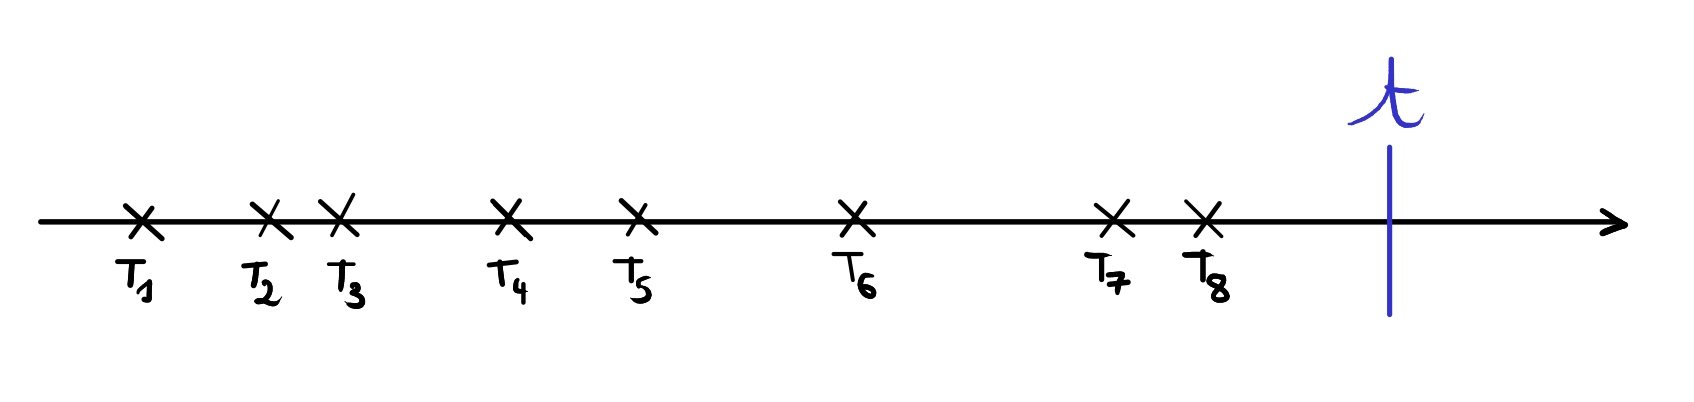
\includegraphics[width=.6\textwidth]{\figcp/Bon24-Hawkes-Fig1}
  $$
 
  \begin{itemize}
    \setlength{\itemsep}{0.5\baselineskip}
    \item $(T_k)_{k \geq 1}$ a random collection of points
    \item Count process $N(t) = \sum_{k \geq 1} \Ibb\{T_k \leq t\}$
    \item Intensity function $\lambda(t)$: immediate probability of observing an event at time $t$
  \end{itemize}

  \bigskip \bigskip \pause
  \paragraph{Examples}
  \begin{itemize}
    \setlength{\itemsep}{0.5\baselineskip}
    \item{Homogeneous Poisson process:} $\lambda(t) \equiv \lambda$
    \item{Heterogeneous Poisson process:} $\lambda(t) =$ deterministic function
    \item{Hawkes process:} $\lambda(t) =$ random function of the past
  \end{itemize}
  
}

%====================================================================
\frame{\frametitle{Segmentation \& classification of a point process} 

  \paragraph{Aim}
  \begin{enumerate}
    \setlength{\itemsep}{0.5\baselineskip}
    \item Propose a set of reasonably realistic models;
    \item Design an (efficient) algorithm to get the parameter estimates;
    \item Choose among the models.
  \end{enumerate}
  
  \bigskip \bigskip \pause
  \paragraph{Example} Segmentation of a Poisson process \refer{DLR23}:
  \begin{enumerate}
    \setlength{\itemsep}{0.5\baselineskip}
    \item Model = Poisson process with piece-wise constant intensity function
    \item Algorithm = dynamic programming in (less than) $\Ocal(N(T)^2)$
    \item Model selection = cross validation (using thining)
  \end{enumerate}

  \bigskip \bigskip \pause
  \paragraph{But} Segmenting a Poisson process
  \begin{enumerate}
    \setlength{\itemsep}{0.5\baselineskip}
    \item Does not fit the scope of RMR2024\footnote{Mod�les statistiques pour des donn�es d�pendantes et applications}
    \item Does not provide any classification (although doable);
    \item Does not account for the the self exciting (or inhibiting) nature of some processes.
  \end{enumerate}

}

%====================================================================
%====================================================================
\section{(Discrete) Hawkes process}
\frame{\frametitle{Outline} \tableofcontents}
\frame{\frametitle{Outline} \tableofcontents[currentsection]}
%====================================================================
\frame{\frametitle{Univariate Hawkes process} 

  $$
  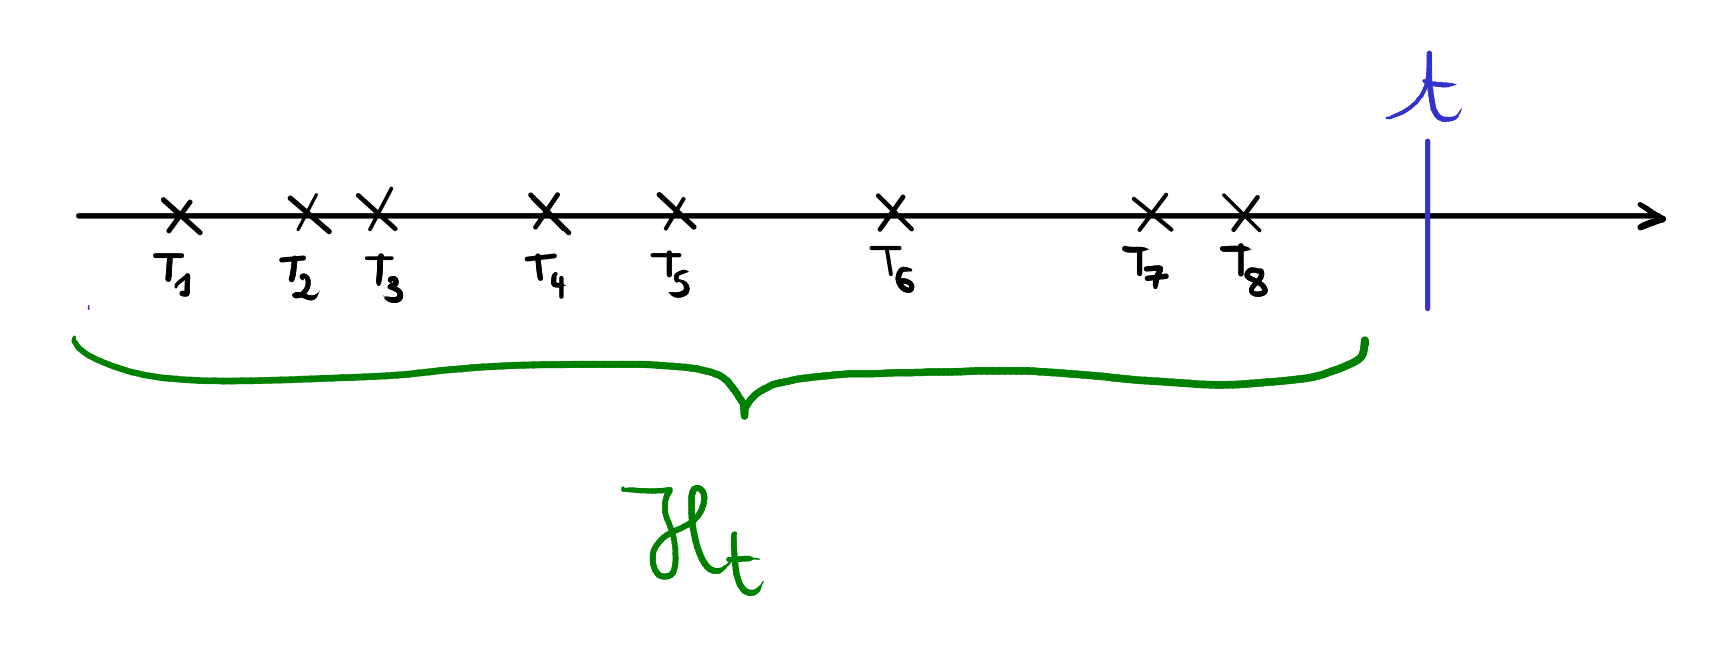
\includegraphics[width=.6\textwidth]{\figcp/Bon24-Hawkes-Fig2}
  $$
 
  \bigskip
  \paragraph{(Conditional) intensity function for the Hawkes process \refer{Haw71a}:}
  $$
  \lambda(t \mid \Hcal_t)= \lambda(t) = \lambda_0 + \underset{T_k < t}{\sum} h(t-T_k)
  $$
 %\nocite{Haw71b}
 
  \begin{itemize}
  \item $\lambda_0 =$ baseline 
  \item $h =$ kernel = influence of past events
  \end{itemize}

}

%====================================================================
\frame{\frametitle{Self-exciting exponential Hawkes process} 

  $$
  \lambda(t)= \lambda_0 + \underset{T_k < t}{\sum} a e^{-b(t-T_k)}
  $$
  \paragraph{Self exciting:} 
  Each event increases the probability of observing another event
  
  \bigskip \bigskip \pause
  \begin{tabular}{cc}
    \hspace{-.04\textwidth}
    \begin{tabular}{p{.4\textwidth}}
      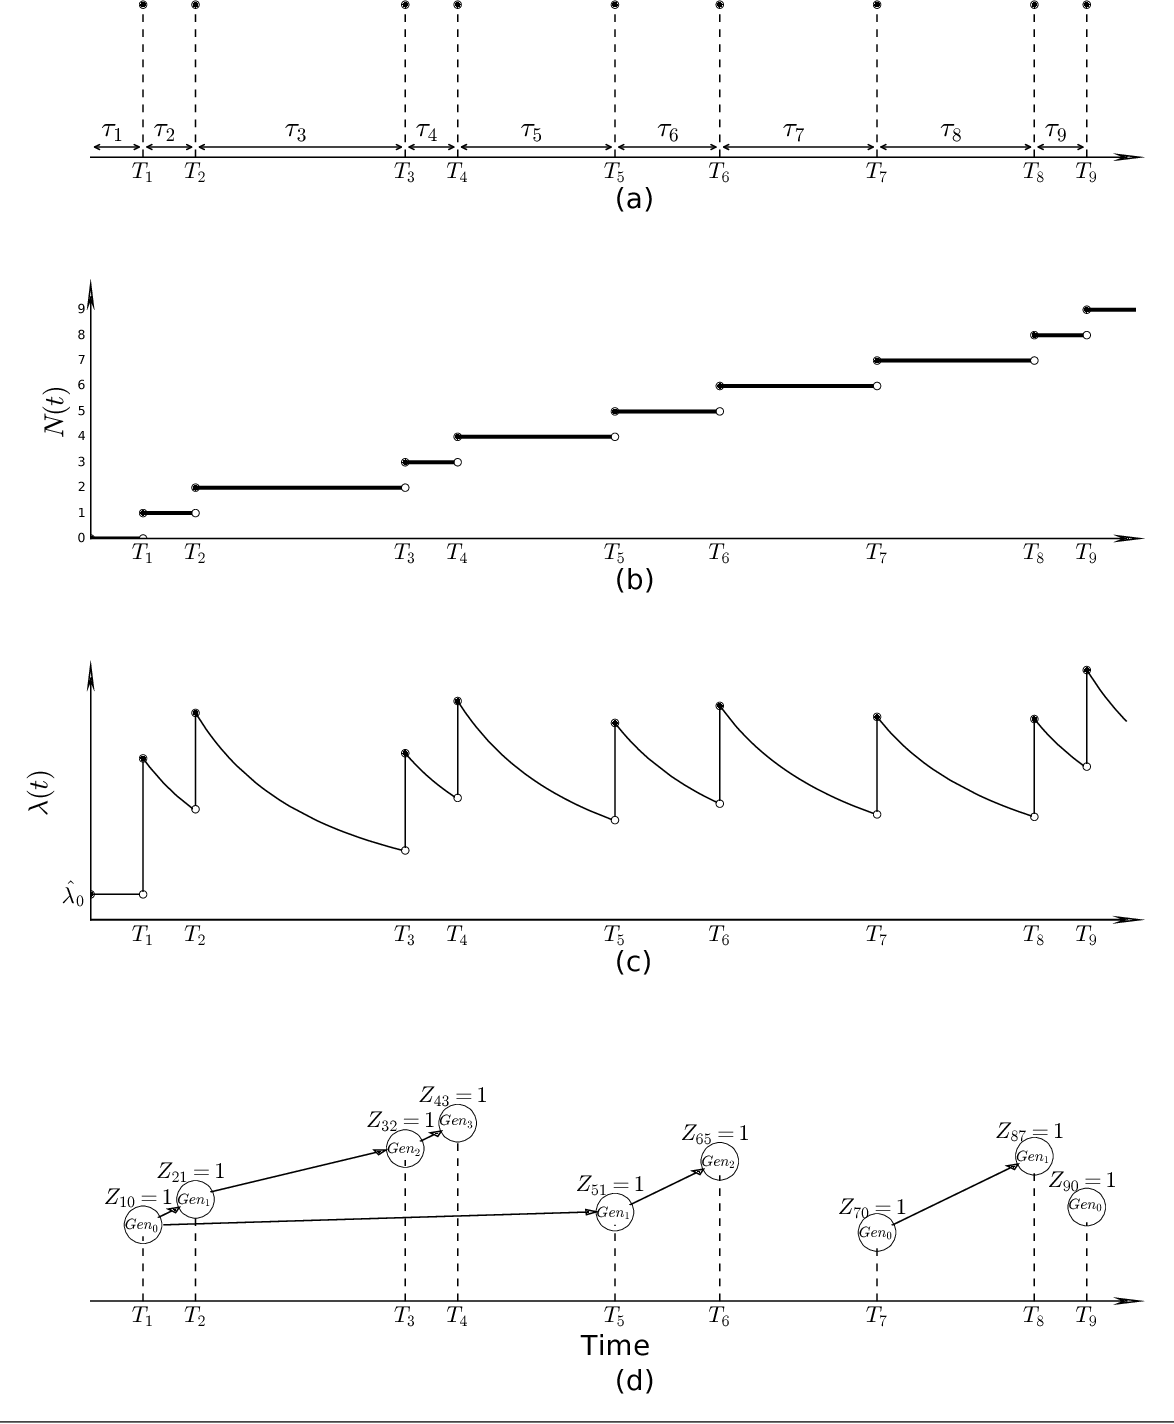
\includegraphics[width=.4\textwidth, trim=0 450 0 0, clip=]{\figcp/Bon24-Hawkes-Fig3}
    \end{tabular}
    & 
    \hspace{-.05\textwidth}
    \begin{tabular}{p{.55\textwidth}}
      \begin{itemize}
        \setlength{\itemsep}{1\baselineskip}
        \item Exponential kernel function \emphase{$h(t)= a e^{-b t}$}
        \item \emphase{$a \geq 0$} to ensure that $\lambda$ is non negative 
        \item \emphase{$a/b <1$} to ensure stationarity
        \item Applications: sismology, epidemiology, neuroscience, ecology, ...
      \end{itemize}
    \end{tabular}
  \end{tabular}  

}

%====================================================================
\frame{\frametitle{Discrete time Hawkes process} 


\paragraph{Continuous time exponential Hawkes process}
$$
\lambda(t)=\lambda_0 + \underset{T_k < t}{\sum} a e^{-b(t-T_k)} 
$$    

\bigskip \bigskip \pause
\paragraph{Discretization}
\begin{itemize}
  \setlength{\itemsep}{0.75\baselineskip}
  \item $I_k=[ \tau_{k-1};\tau_k]$ with $\tau_k=k\Delta$
  \item $N_k=N(I_k)$ the number of events on $I_k$
  $$
  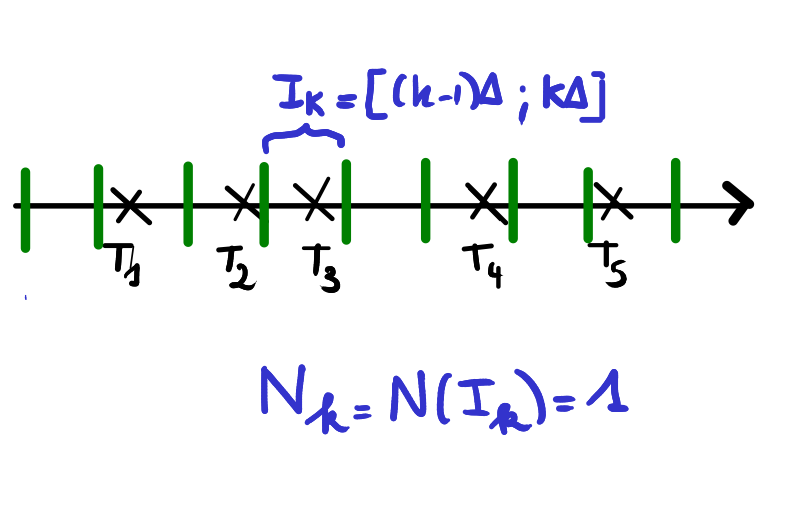
\includegraphics[width=.45\textwidth, trim=0 230 0 70, clip=]{\figcp/Bon24-Hawkes-Fig4}
  $$
  \item Distribution of $(N_k)_{k \geq 1}$?
\end{itemize}

}

%====================================================================
\frame{\frametitle{Cluster representation} 

  $$
  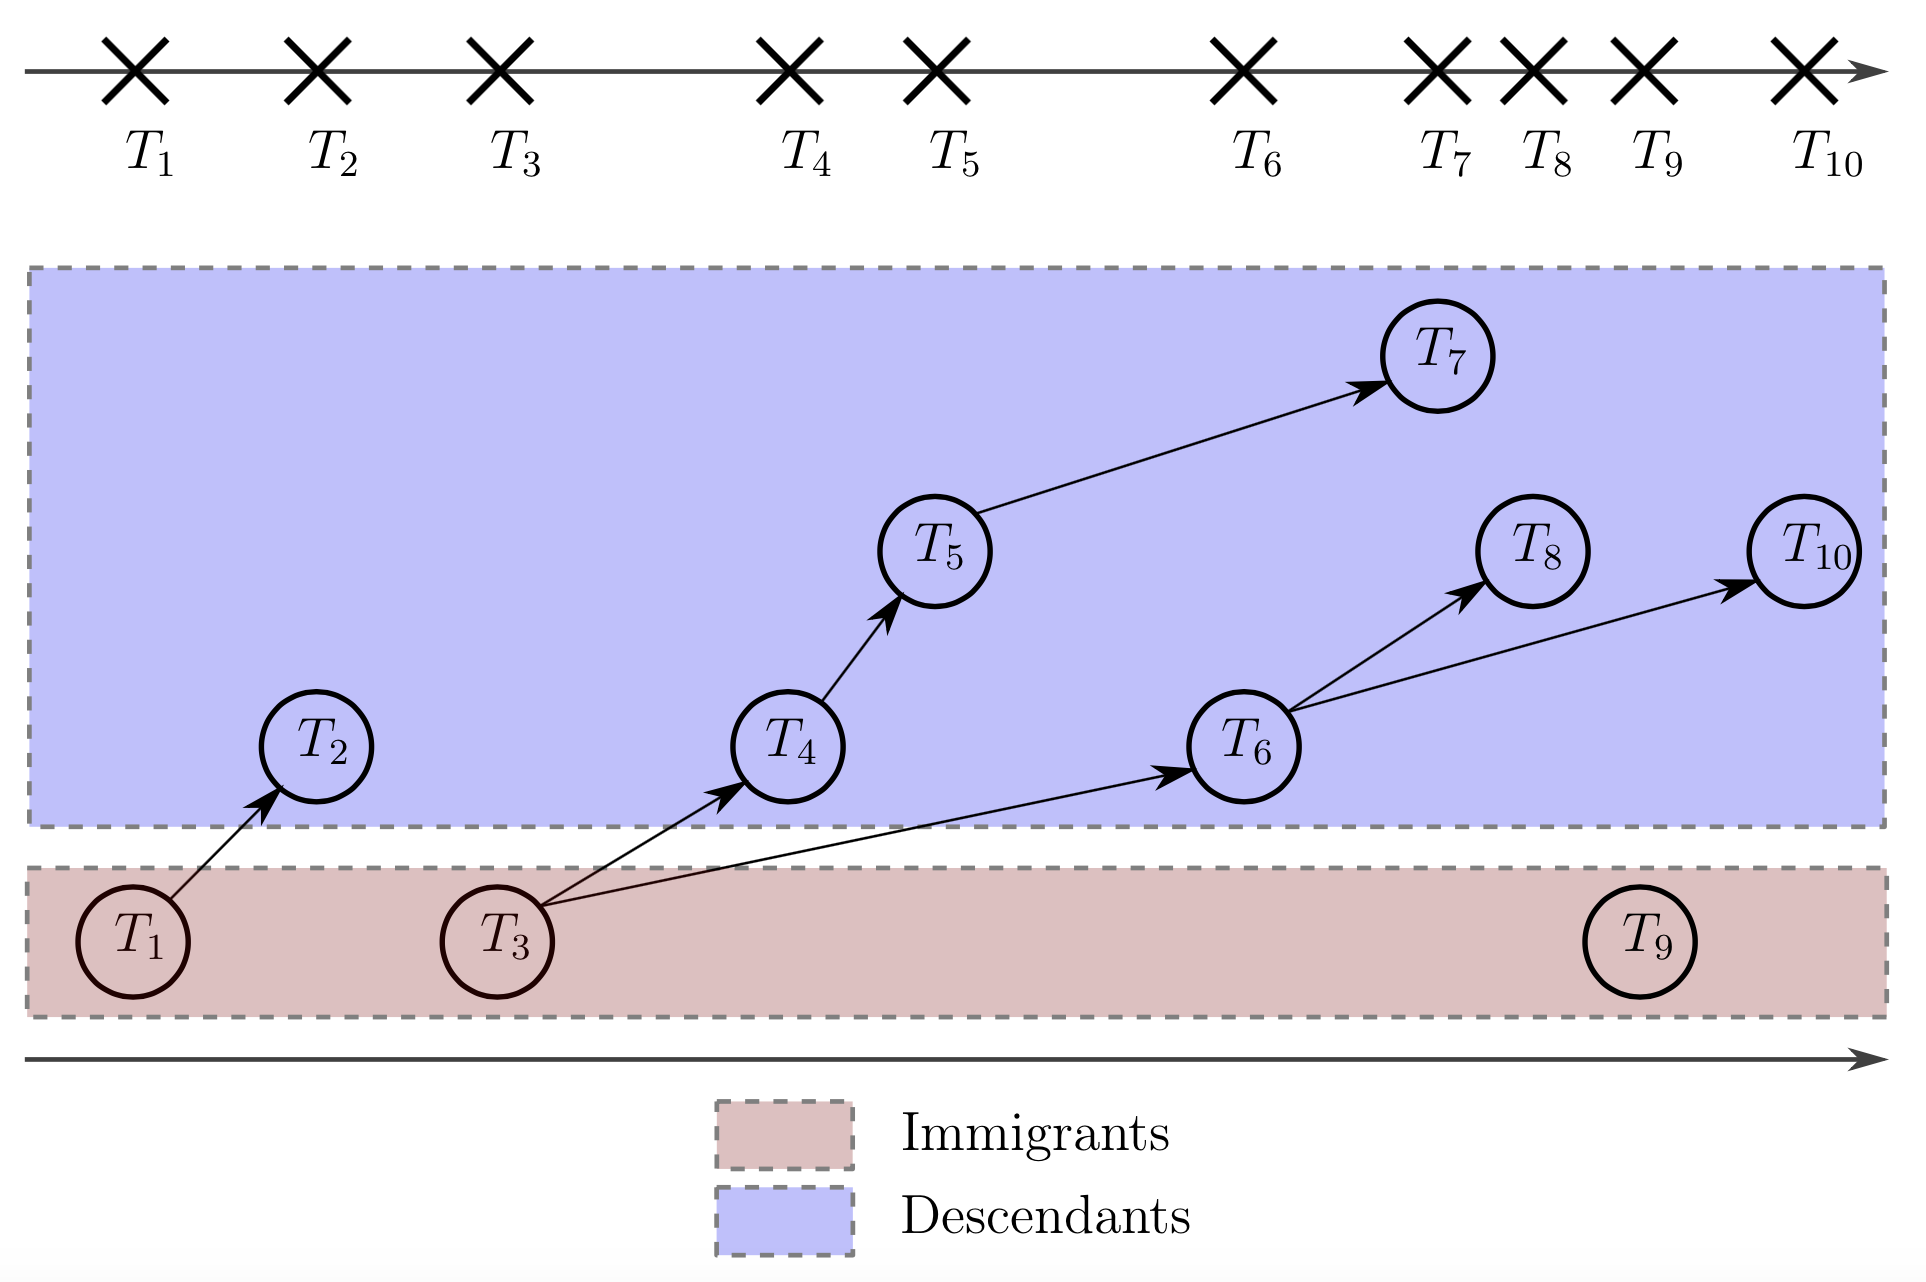
\includegraphics[width=.7\textwidth]{\figcp/Bon24-Hawkes-Cluster}
  $$

  \begin{itemize}
  \item Immigrants arrive at rate $\lambda_0$ 
  \item Each immigrant or descendant produces new individuals at rate $h(t - T)$
  \end{itemize}

}

%====================================================================
\frame{\frametitle{Discrete time Hawkes process} 

  $N_k=N(I_k)$ the number of events on $I_k=[ \tau_{k-1};\tau_k]$
  
  \bigskip \bigskip \pause
  \paragraph{Count distribution}
  $$
  N_k \overset{\Delta}{=} B_k + \sum_{\ell \leq k-1} \sum_{T \in I_\ell} M_T(I_k) + R_k
  $$
  \begin{itemize}
    \item $B_k \sim \mathcal{P}(\lambda_0 \Delta)$ discrete immigrant process
    \item $ M_T(I_k) \sim \mathcal{P}\left(c(a,b,\Delta) e^{-b(\tau_{k-1}-\emphase{T})}\right)$ descendants of $T<\tau_{k-1}$
    \item $R_k$ number of descendants of points $T \in I_k$ within $I_k$
  \end{itemize}

  \bigskip \bigskip \pause
  \paragraph{Approximation when $\Delta$ is small}
  \begin{itemize}
    \item  $ M_T(I_k) \simeq \mathcal{P}\left(c(a,b,\Delta) e^{-b(\tau_{k-1}-\emphase{\tau_{\ell-1}})}\right)$ for $T \in  I_\ell=[\tau_{\ell-1}; \tau_\ell]$
    \item \emphase{$R_k \simeq 0$}
  \end{itemize}
}

%====================================================================
\frame{\frametitle{Markovian reformulation} 

  \paragraph{Approximation of $N_k$}
  $$
  Y_k \mid \{Y_\ell\}_{\ell \leq k-1} \sim \mathcal{P}\left(\mu + \sum_{\ell = 1}^{\infty} \alpha \beta^\ell Y_{k-\ell} \right),
  $$
  with $\mu=\lambda_0 \Delta$ and $\alpha$, $\beta$ depending on $a$, $b$, $\Delta$.

  \bigskip \bigskip \pause
  \paragraph{$\{Y_k\}_{k\geq 1}$ is not a Markov chain but...} 
  Let us define $(U_k)_{k \geq 1}$
  $$
  U_1 = 0, \qquad
  U_k = \alpha Y_{k-1} + \beta U_{k-1}, 
  $$
  so that
  $$
  Y_k \vert (U_{k-1}, Y_{k-1}) \sim  \mathcal{P}\left(\alpha Y_{k-1} +  \beta U_{k-1} \right),
  $$   
  we have that
  $$
  \left((Y_k,U_k)\right)_{k \geq 1} \text{ is a Markov Chain}
  $$

}

%====================================================================
%====================================================================
\section{Discrete Markov switching Hawkes process}
\frame{\frametitle{Outline} \tableofcontents[currentsection]}
%====================================================================
\frame{\frametitle{Discrete time Hawkes HMM} 

  \paragraph{Model:} $Q$ hidden states
  \begin{itemize}
  \item Hidden path: $\{Z_k\}_{k \geq 1}$ homogeneous Markov chain with transition matrix $\pi$
  \item Observed counts: for $k\geq 1$, set $U_1=0$ and
    $$
    Y_k \mid \{Y_\ell\}_{\ell \leq k-1} 
    \sim \mathcal{P}\left(\emphase{\mu_{Z_k}} + \sum_{\ell = 1}^{\infty} \alpha \beta^\ell Y_{k-\ell} \right)
    $$  
  \end{itemize}
  \paragraph{Graphical model:}
  \begin{figure}
    \begin{centering}
    \begin{tikzpicture}
\node[] (Zt_2) at (-\edgeunit, \edgeunit) {}; 
\node[] (Zt_1) at (0, \edgeunit) {$Z_{k-1}$}; 
\node[] (Zt) at (\edgeunit, \edgeunit) {$Z_{k}$}; 
\node[] (Zt1) at (2*\edgeunit, \edgeunit) {$Z_{k+1}$}; 
\node[] (Zt2) at (3*\edgeunit, \edgeunit) {}; 
\node[] (Ut_1) at (-0.5*\edgeunit, 0.5*\edgeunit) {$U_{k-1}$}; 
\node[] (Ut) at (0.5*\edgeunit, 0.5*\edgeunit) {$U_{k}$}; 
\node[] (Ut1) at (1.5*\edgeunit, 0.5*\edgeunit) {$U_{k+1}$}; 
\node[] (Ut2) at (2.5*\edgeunit, 0.5*\edgeunit) {$U_{k+2}$}; 
\node[] (Ut3) at (3.5*\edgeunit, 0.5*\edgeunit) {}; 
\node[] (Yt_2) at (-\edgeunit, 0) {}; 
\node[] (Yt_1) at (0, 0) {$Y_{k-1}$}; 
\node[] (Yt) at (\edgeunit, 0) {$Y_{k}$}; 
\node[] (Yt1) at (2*\edgeunit, 0) {$Y_{k+1}$}; 
\node[] (Yt2) at (3*\edgeunit, 0) {}; 

\draw[->,dashed] (Zt_2) -- (Zt_1); \draw[->] (Zt_1) -- (Zt); \draw[->] (Zt) -- (Zt1); \draw[->,dashed] (Zt1) -- (Zt2);
\draw[->] (Zt_1) -- (Yt_1); \draw[->] (Zt) -- (Yt); \draw[->] (Zt1) -- (Yt1);
\draw[->] (Ut_1) -- (Yt_1); \draw[->] (Ut) -- (Yt); \draw[->] (Ut1) -- (Yt1);
\draw[->] (Ut_1) -- (Ut); \draw[->] (Ut) -- (Ut1); \draw[->] (Ut1) -- (Ut2); \draw[->,dashed] (Ut2) -- (Ut3);
\draw[->,dashed] (Yt_2) -- (Ut_1); \draw[->] (Yt_1) -- (Ut); \draw[->] (Yt) -- (Ut1); \draw[->] (Yt1) -- (Ut2);
\end{tikzpicture}

    \end{centering}
  \end{figure}

  \bigskip \pause
  \paragraph{Assumptions:}
  \begin{itemize}
    \item The immigration rate varies with the hidden path
    \item The number of offspring does not vary with the hidden path
  \end{itemize}

}

%====================================================================
\frame{\frametitle{Inference}

  \paragraph{Aim:} Infer the parameter $\theta = ((\mu_q)_{1 \leq q \leq Q}, \pi)$
  $$
  \widehat{\theta} = \log p_\theta(Y)
  $$

  \bigskip \pause
  \paragraph{EM algorithm:} \refer{DLR77}
  $$
  \theta^{(h+1)} 
  = \underset{\text{\normalsize \emphase{M step}}}{\underbrace{\argmax_\theta}} \; \underset{\text{\normalsize \emphase{E step}}}{\underbrace{\Esp_{\theta^{(h)}}}}[\log p_\theta(Y, Z) \mid Y]
  $$
  \begin{itemize}
    \setlength{\itemsep}{.75\baselineskip}
    \item E step: Evaluate $\ell^{(h)}(\theta) = \Esp_{\theta^{(h)}}[\log p_\theta(Y, Z) \mid Y]$ (forward-backward recursion)
    \item M step: Gradient descent, computing $\nabla_\theta \ell^{(h)}(\theta)$ by recursion
  \end{itemize}

  \bigskip \bigskip \pause
  \paragraph{By-product:} Classification
  $$
  \widehat{Z}_k = \argmax_q P_{\widehat{\theta}}\{Z_k = q \mid Y \}, 
  \qquad
  \widehat{Z} = \argmax_z p_{\widehat{\theta}}(Y, Z=z) 
  $$

}

%====================================================================
\frame{\frametitle{Synthetic data: classification} 

\begin{center}
  \begin{tabular}{c||c|cccc}
    & States &  1 &2  & 3\\
    \hline
    \multirow{3}{*}{Hawkes HMM}& 1 & 273.7 & 28.7 & 14.2\\
    & 2 &  37 & 166.3 & 96.9\\
    & 3 &  4.7  & 24.7 & 353.8 \\
    \hline 
    \hline
    \multirow{3}{*}{Poisson HMM}& 1 & 181 & 122.8 & 12.8\\
    &2 &  136 & 111.1 & 53.1\\
    & 3 &  45.4 & 115.2 & 222.6
  \end{tabular} 

  \vspace{0.01\textheight}
  \begin{tabular}{cc}
    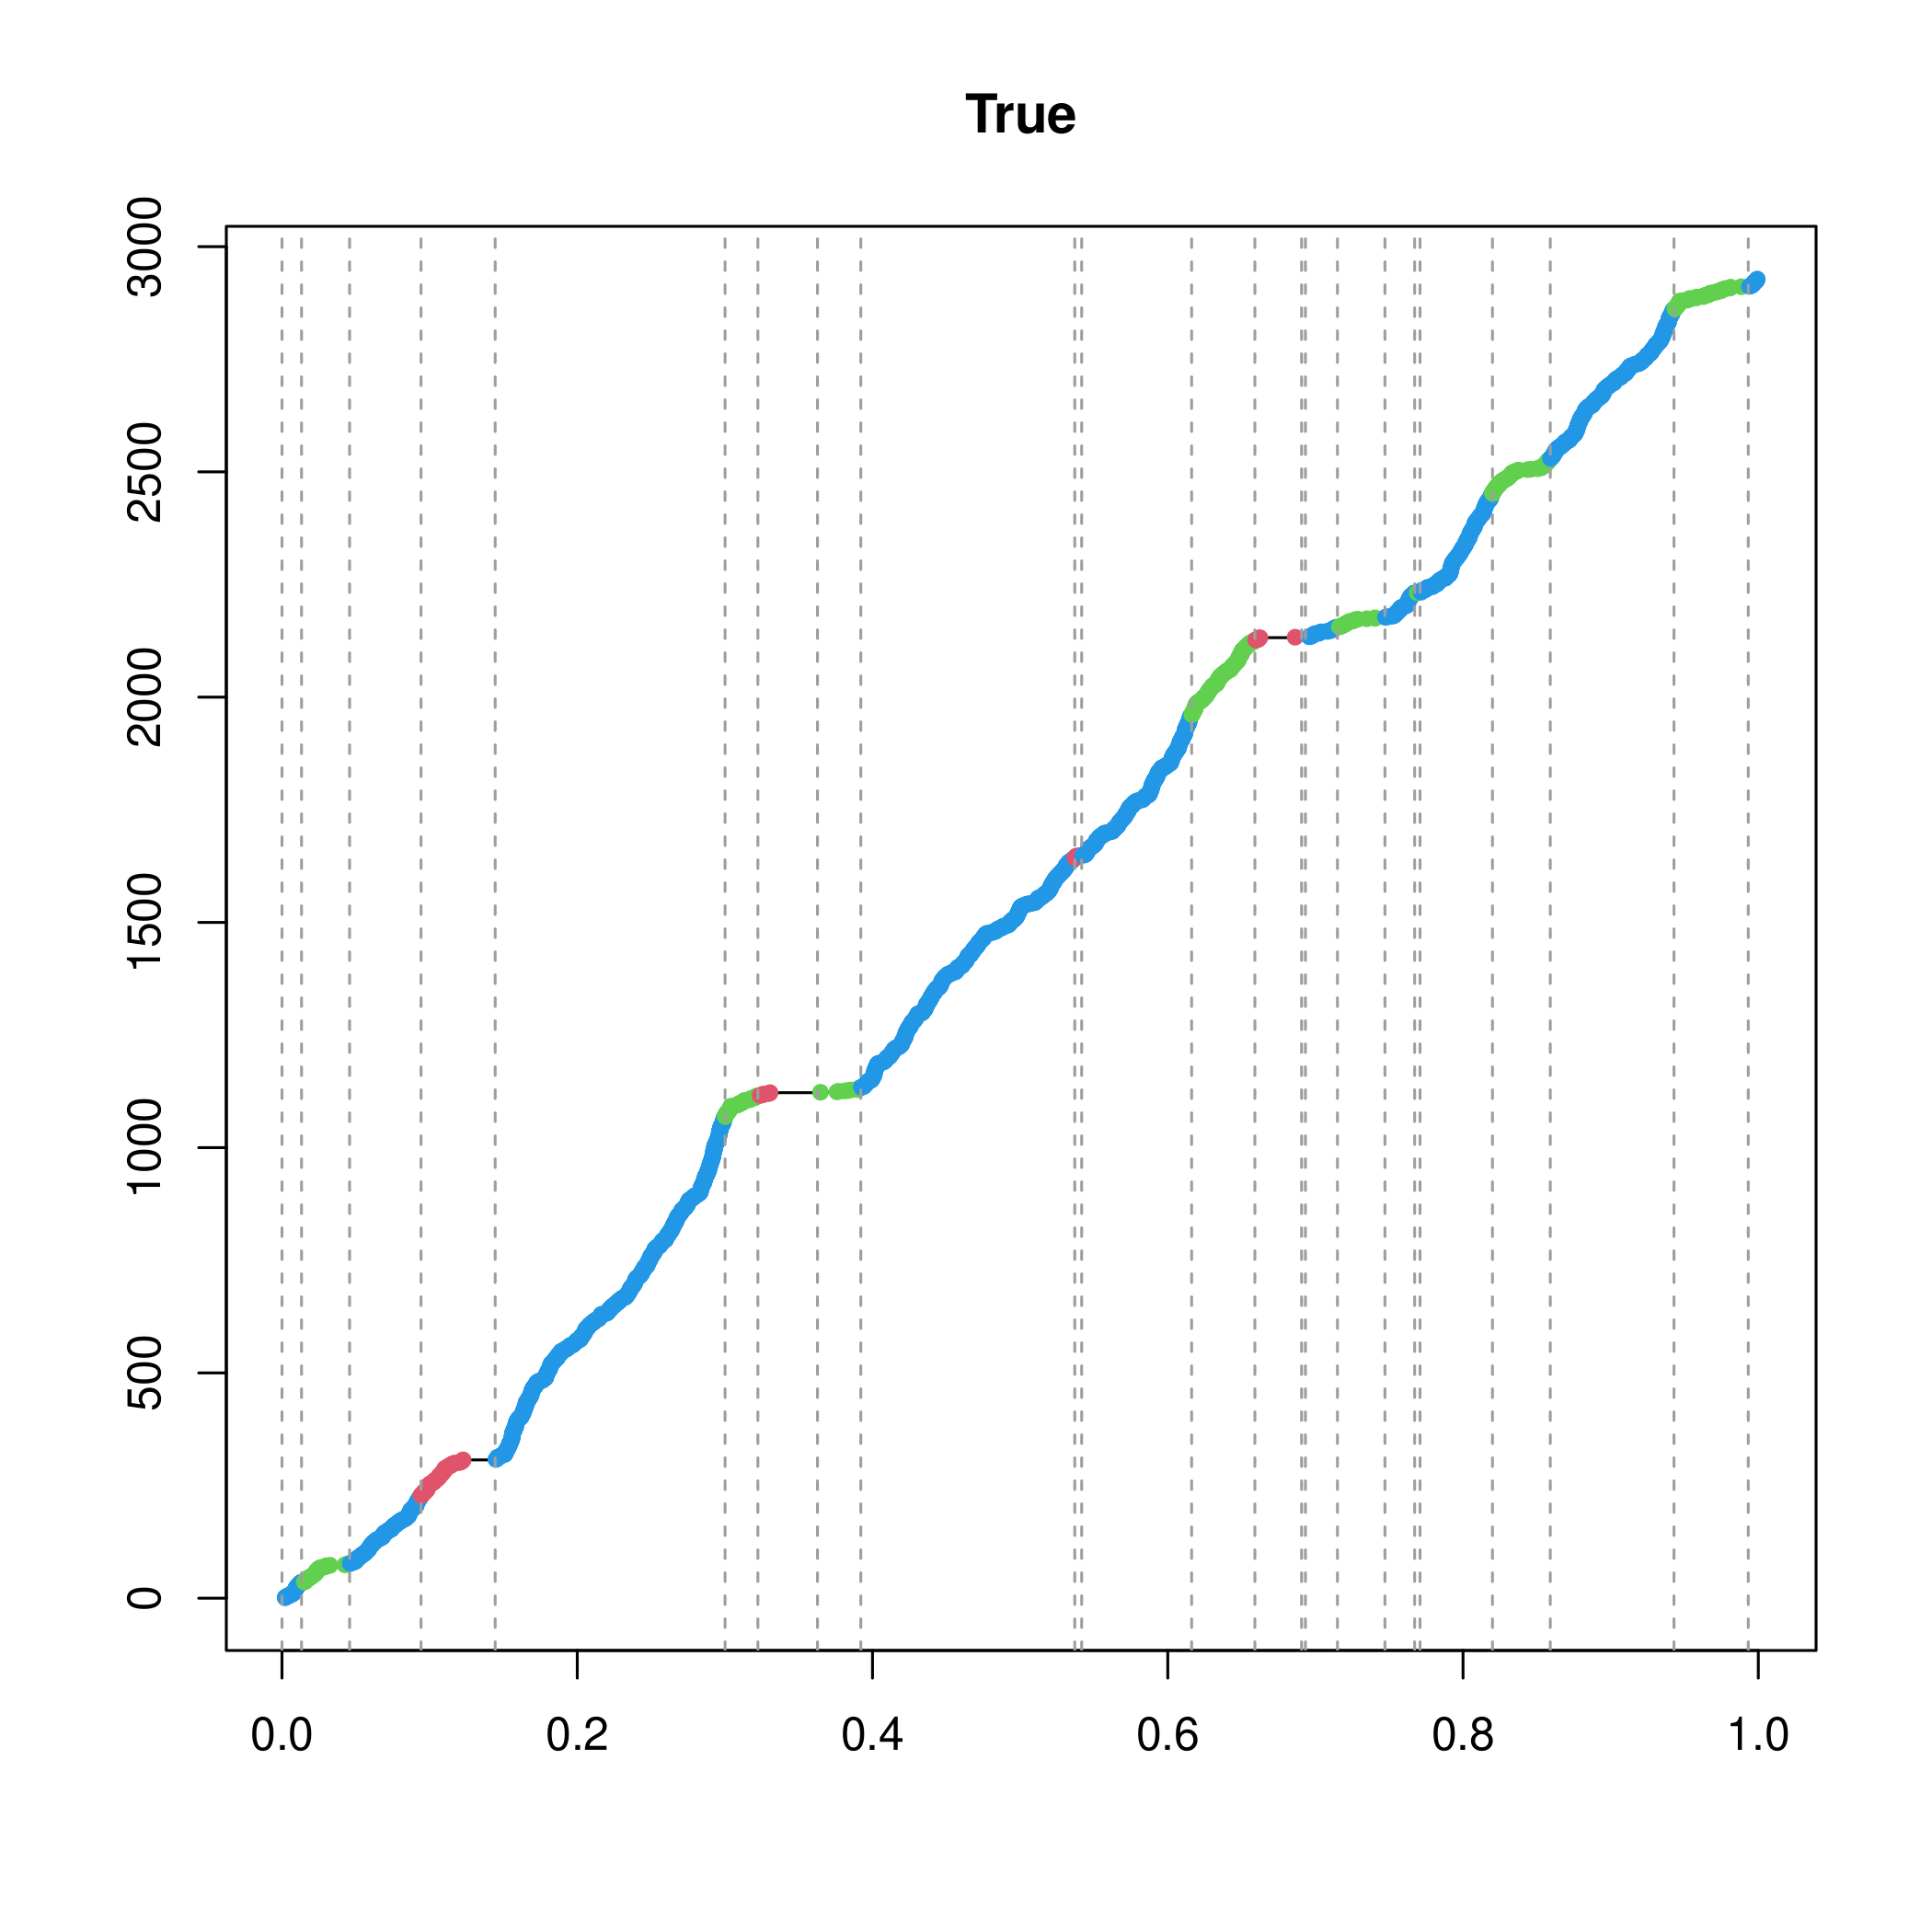
\includegraphics[scale=0.25]{\figcp/Bon24-Hawkes-Fig5a}    & 
    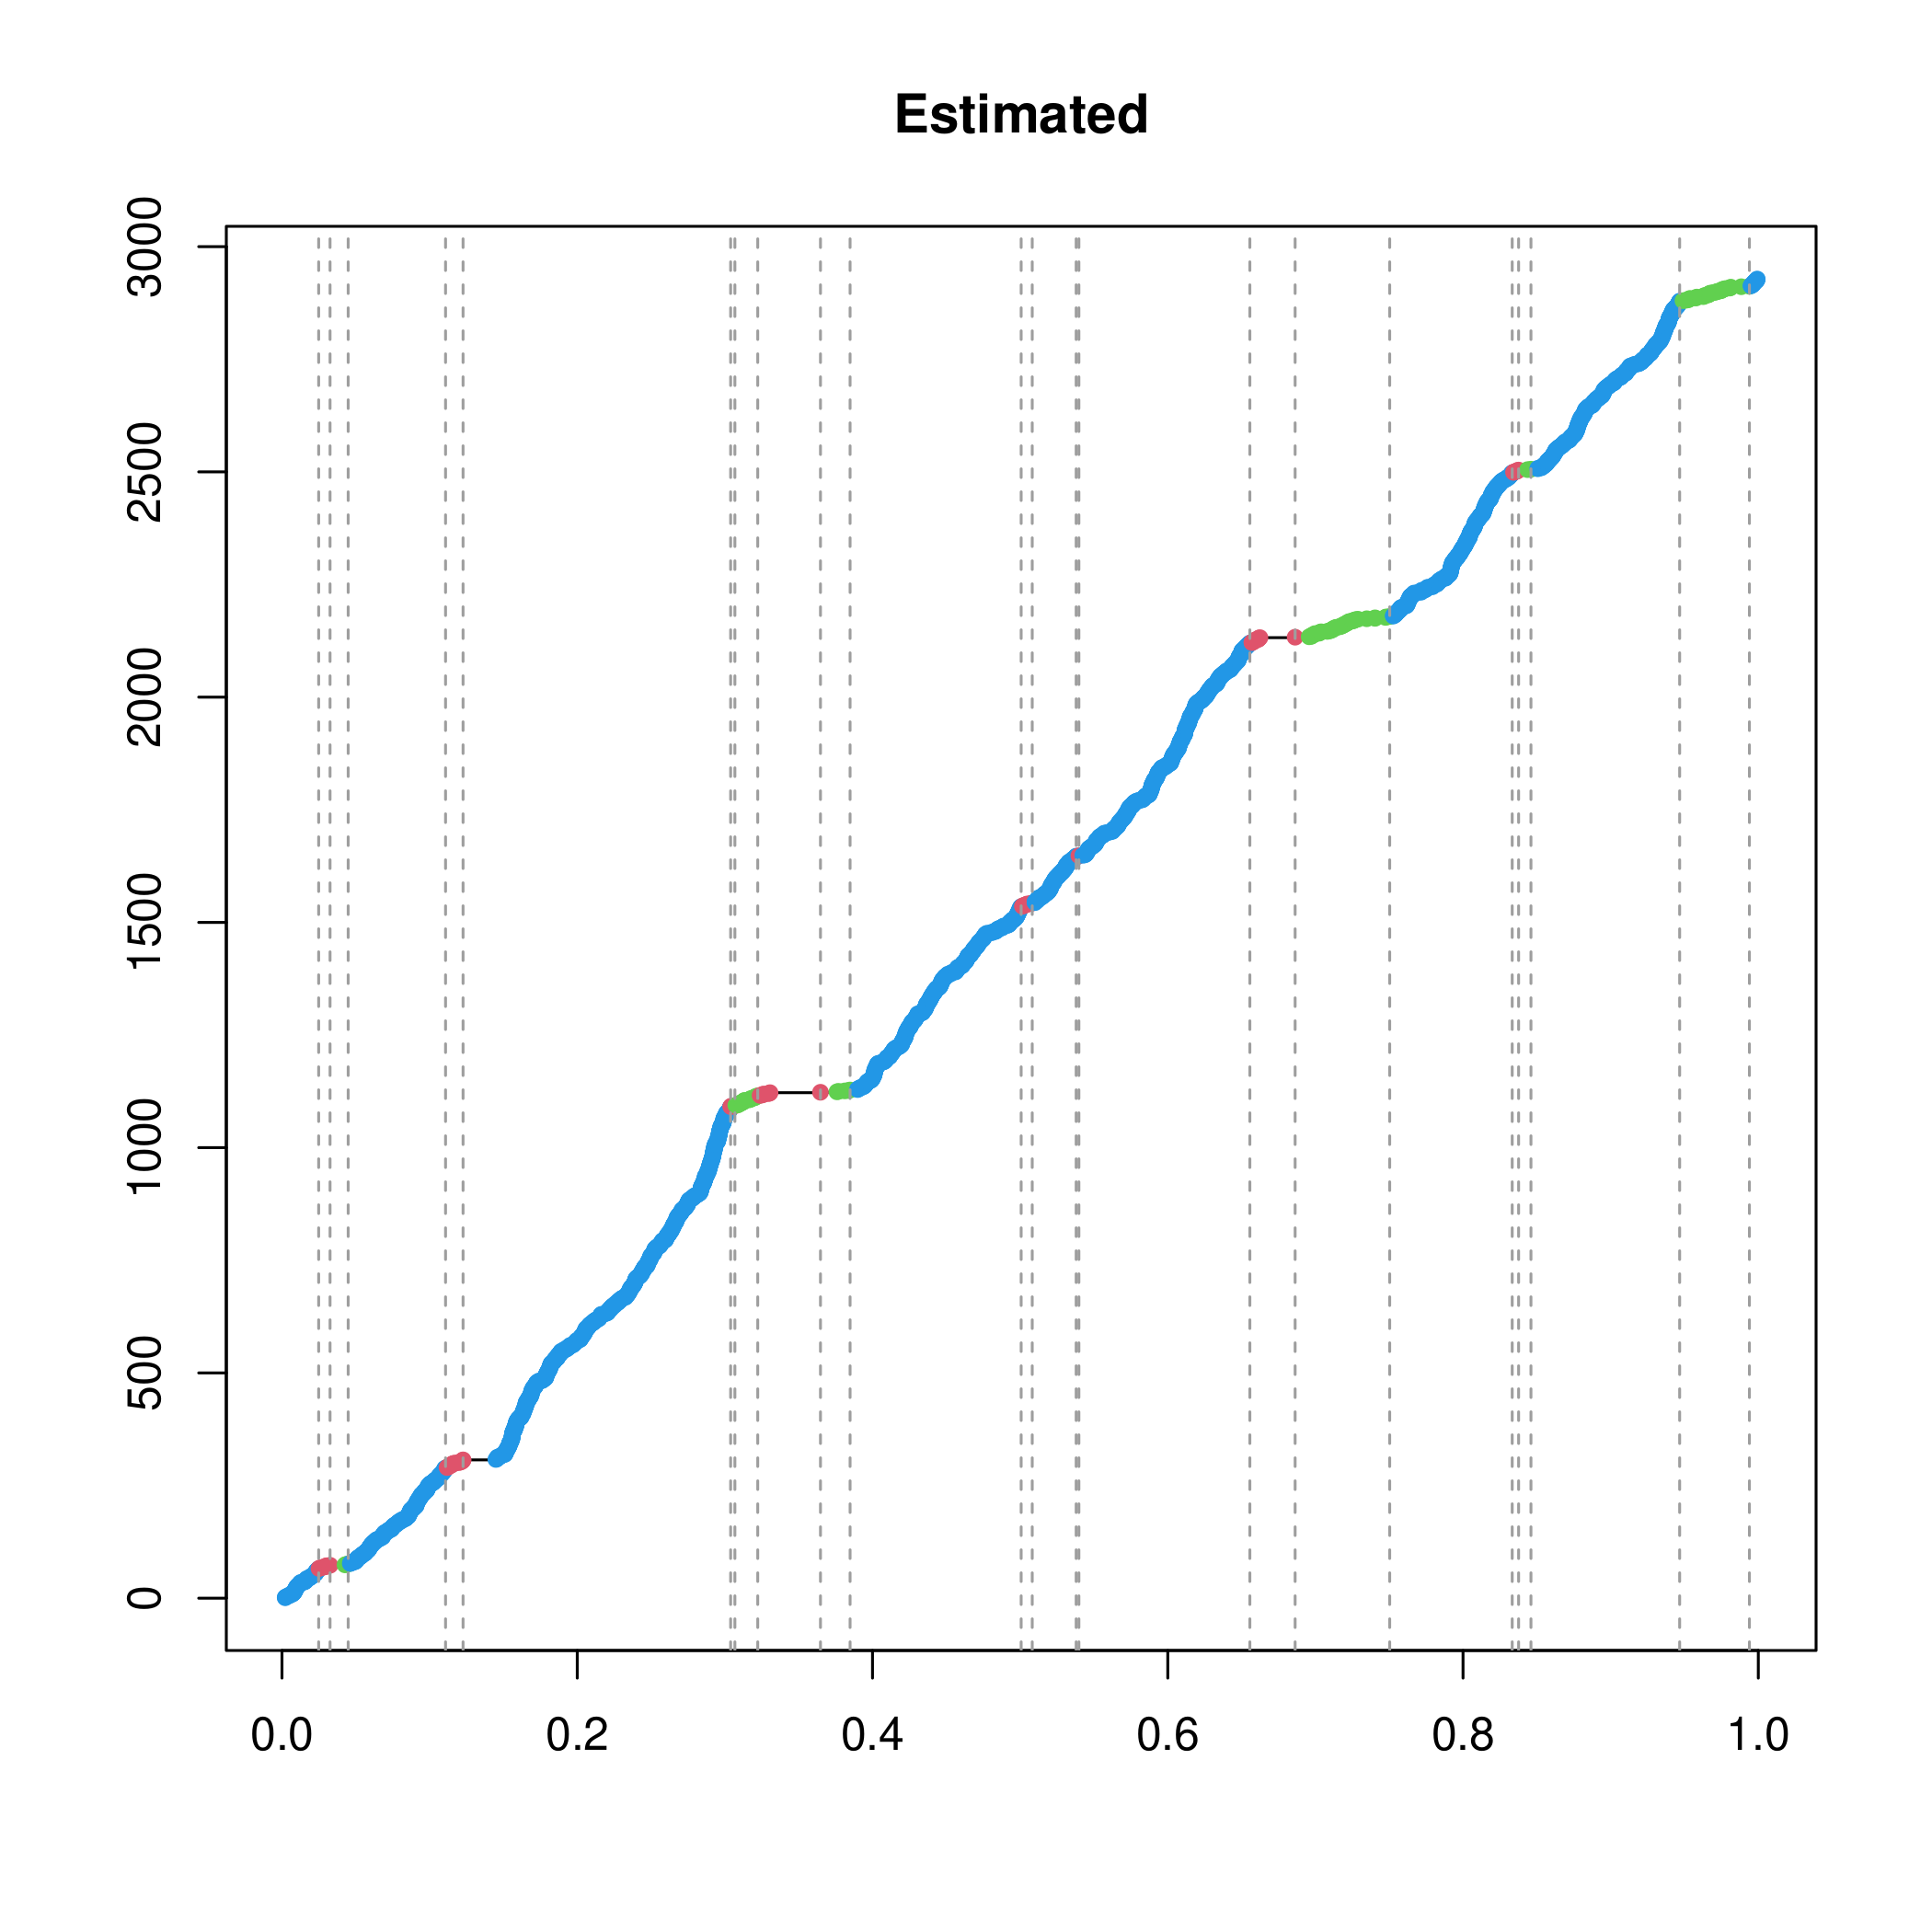
\includegraphics[scale=0.25]{\figcp/Bon24-Hawkes-Fig5b}
  \end{tabular}
\end{center}


}

%====================================================================
\frame{\frametitle{Synthetic data: parameter estimation} 

  $$
  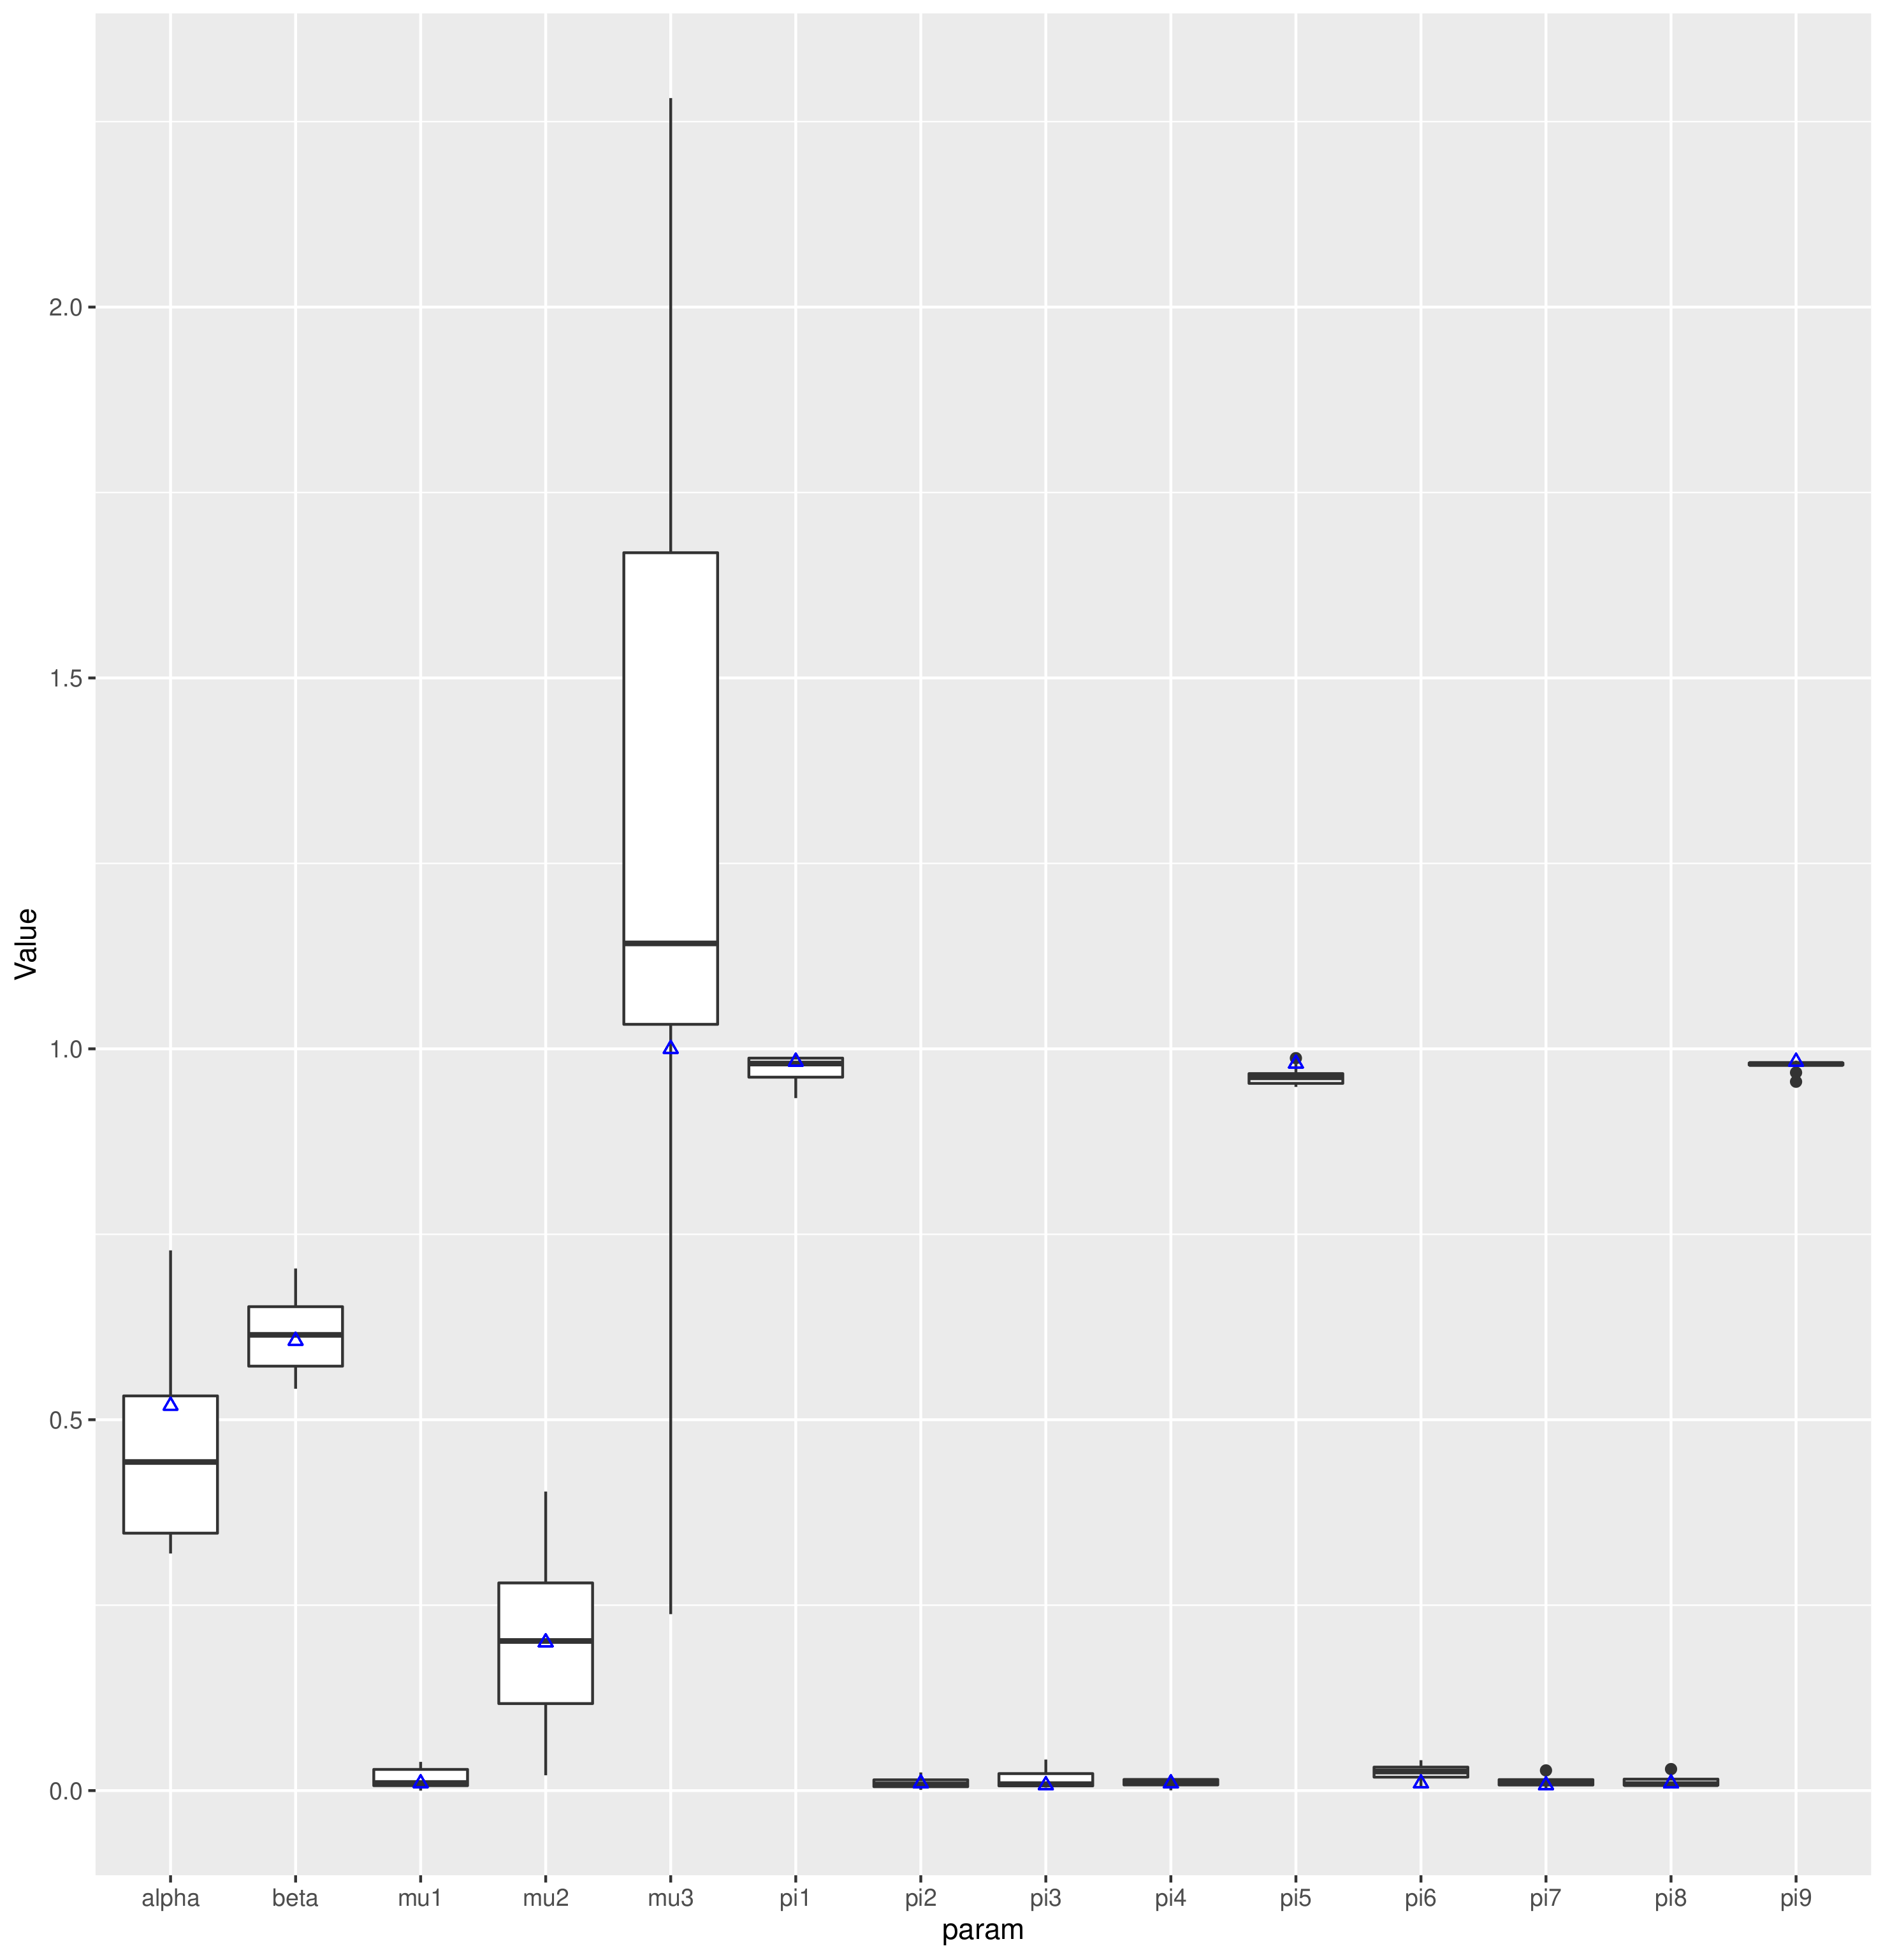
\includegraphics[width=.5\textwidth]{\figcp/Bon24-Hawkes-Fig6}
  $$

}

%====================================================================
\frame{\frametitle{} 

}

%====================================================================
%====================================================================
\section{Goodness of fit}
\frame{\frametitle{Outline} \tableofcontents[currentsection]}
%====================================================================
\frame{\frametitle{Model selection} 

  \paragraph{Aim:} select the number of hidden states $Q$
  
  \bigskip \bigskip \pause
  \paragraph{Penalized likelihood:}
  $$
  \log p_\theta(Y) = \Esp_\theta[\log p_\theta(Y, Z) \mid Y] + \Hcal(p_\theta(Z \mid Y))
  $$
  
  \bigskip 
  \ra Standard criterion for discrete time HMM
  \begin{align*}
    BIC(Q) & = \log p_{\widehat{\theta}_Q}(Y) - pen(\widehat{\theta}_Q), \\
    ICL(Q) & = \log p_\theta(Y)- \Hcal(p_{\widehat{\theta}_Q}(Z \mid Y)) - pen(\widehat{\theta}_Q)
  \end{align*}
  with
  $$
  pen(\widehat{\theta}_Q) = \frac12 \log(N) (Q^2 + 2)
  $$
  where $N =$ number of time steps (i.e. discretized intervals)
}

%====================================================================
\frame{\frametitle{Goodness-of-fit} 

  \paragraph{Time-change theorem \refer{DaV03}}
  A sequence $(T_k)_{k\ge 1}$ is a realization of $N$ if and only if $(\Lambda(T_k))_{k \ge 1}$ is a realization of a homogeneous Poisson process with unit intensity.
  where $$\Lambda(t)=\int_0^t \lambda(u) du \quad \quad \quad \text{(Compensator)}$$

  \bigskip \pause 
  \paragraph{Goodness-of-fit test}
  \begin{itemize}
  \item $H_0$: ``$(T_k)_{k\ge 1}$ is a realization of a HMM-Hawkes process with parameter $\theta$''.
  \item Kolmogorov-Smirnov test between 
  $$
  \left( \Lambda_{\widehat{\theta}}(T_{k+1}) - \Lambda_{\widehat{\theta}}(T_k) \right)_{k \ge 1}
  $$
  and an exponential distribution $\mathcal{E}(1)$.
  \end{itemize}

  \bigskip \bigskip 
  \paragraph{Comments}
  \begin{itemize}
   \item Same test for alternative models (Hawkes, HMM-Poisson)
   \item Train/test samples (resampling procedure, \refer{RRG14}) 
  \end{itemize}

}

%====================================================================
\frame{\frametitle{Synthetic data: Goodness-of-fit (1/2)}

  \begin{center}
    \begin{tabular}{cc}
      \begin{tabular}{p{.45\textwidth}}
      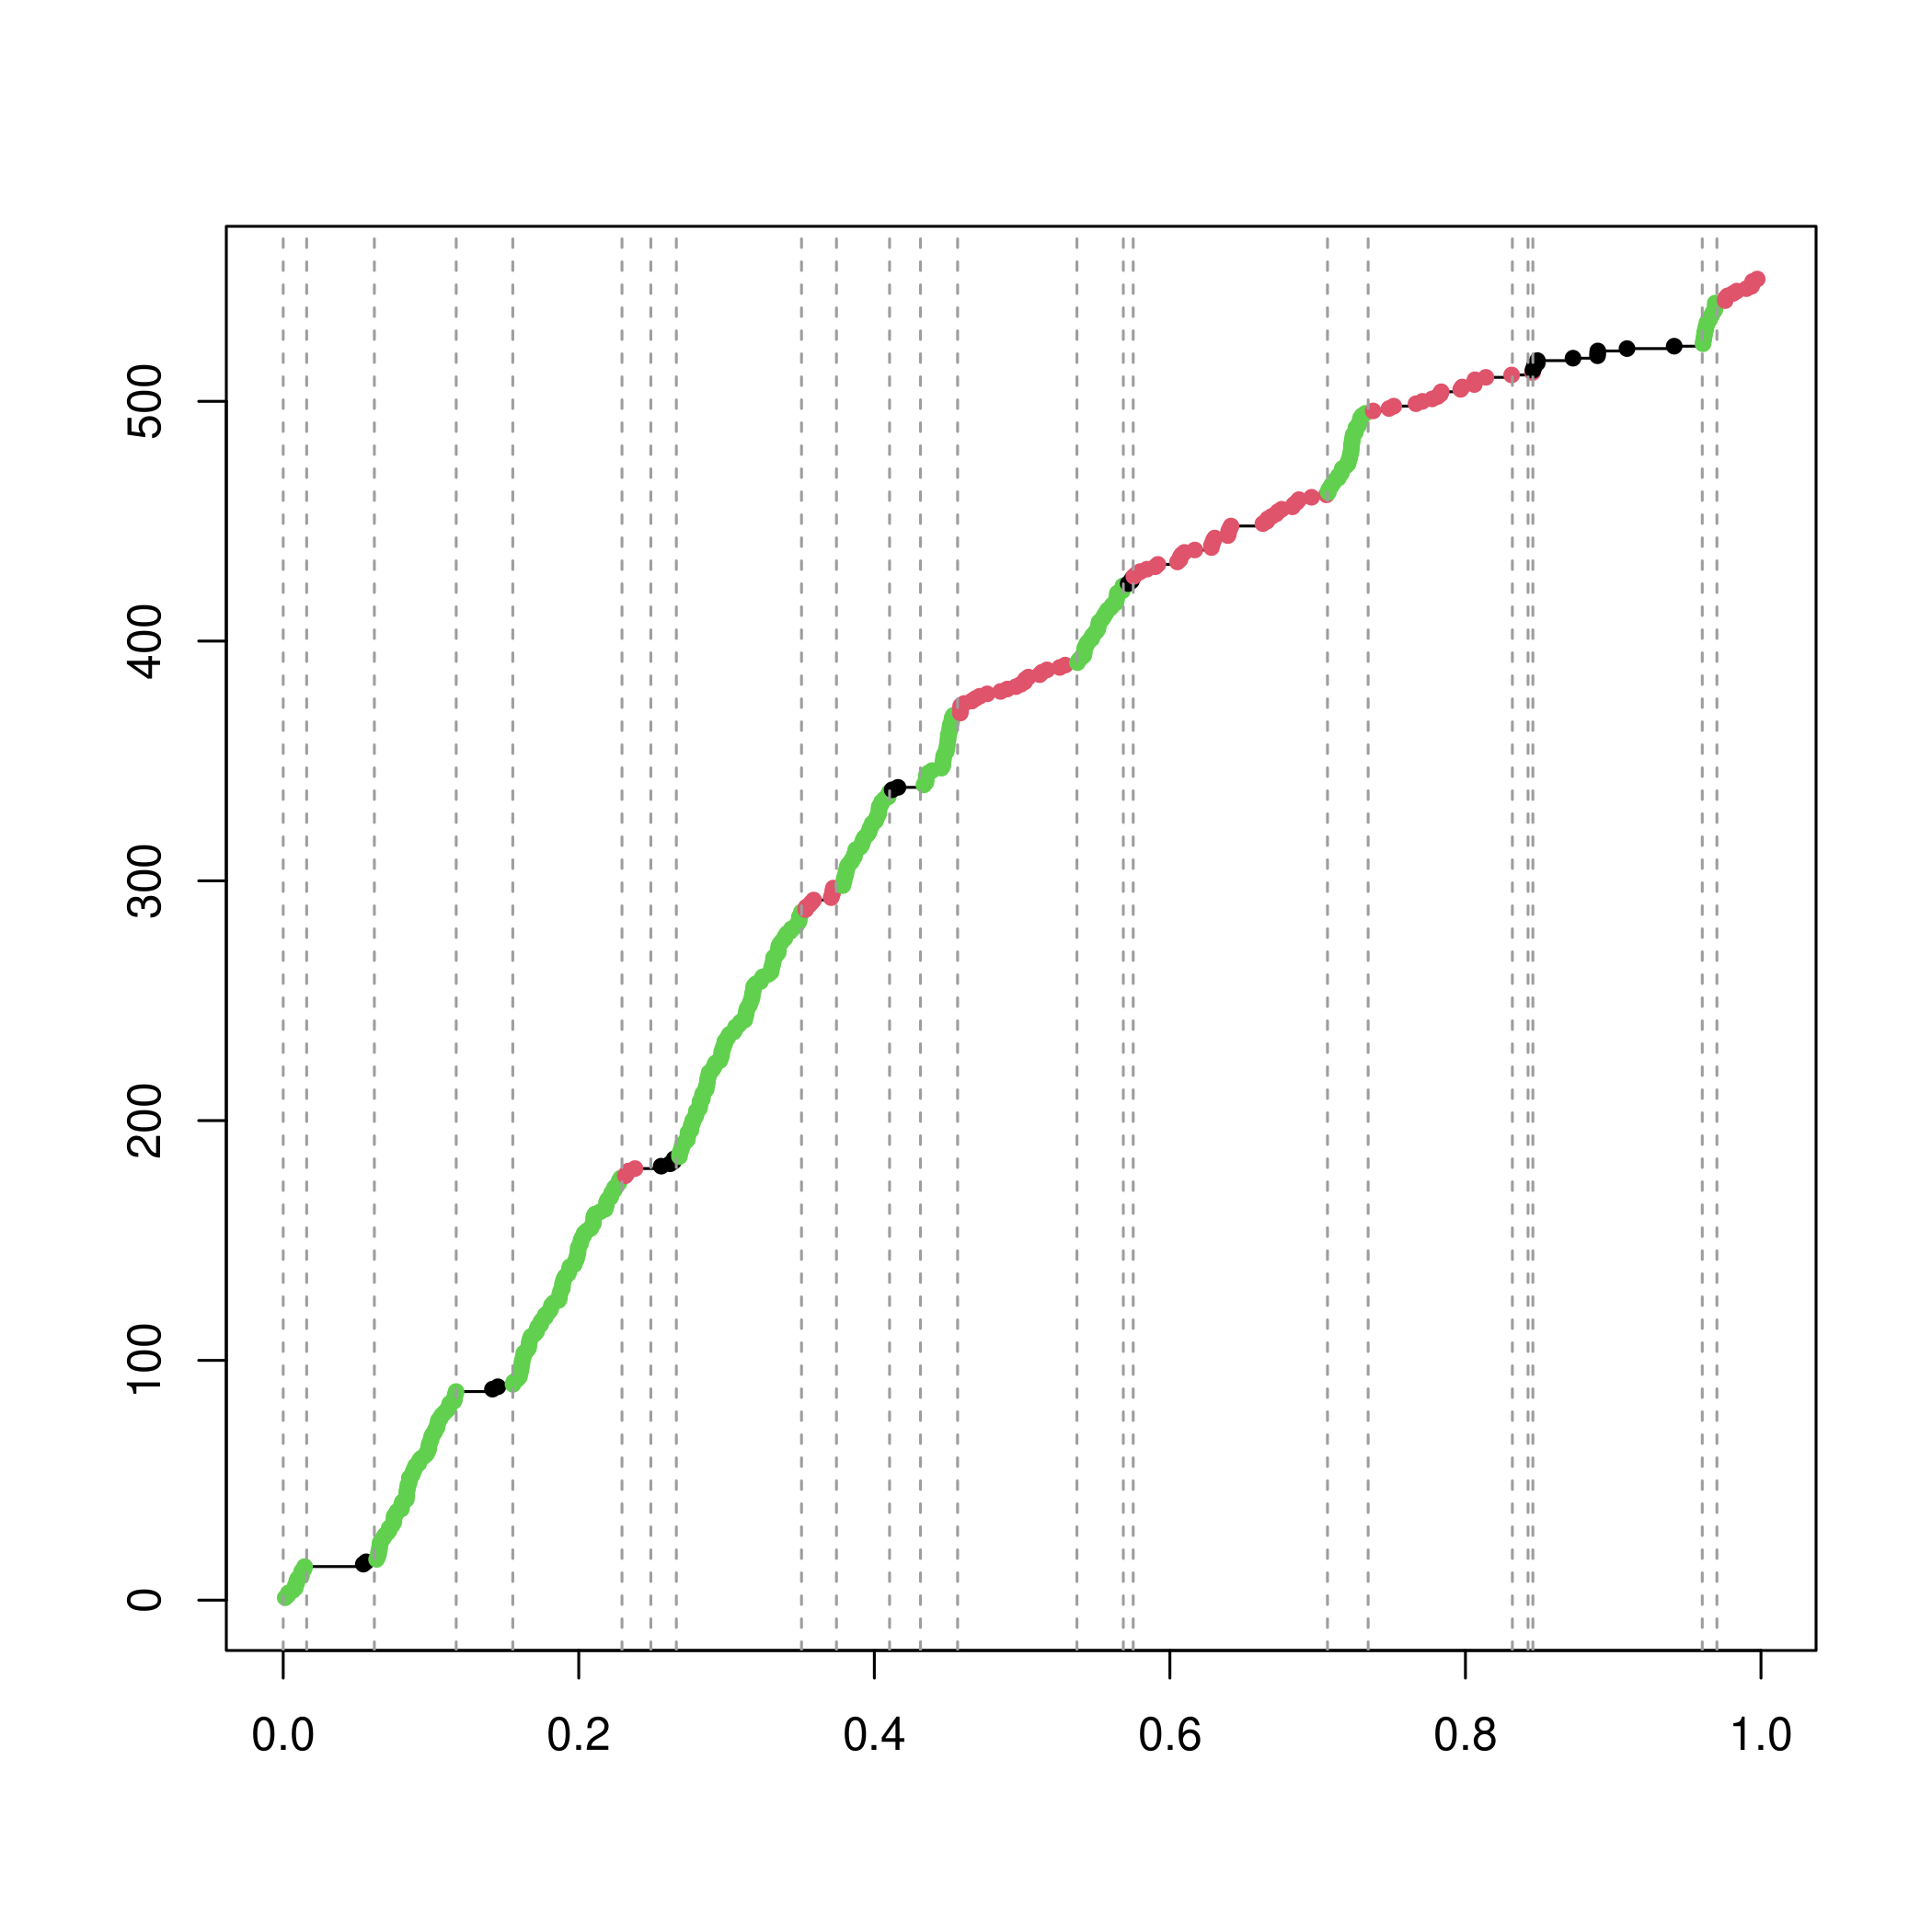
\includegraphics[width=.4\textwidth]{\figcp/Bon24-GOF-Ex1-Path}
      \end{tabular}
      &
      \vspace{-.05\textwidth}
      \begin{tabular}{p{.45\textwidth}}
      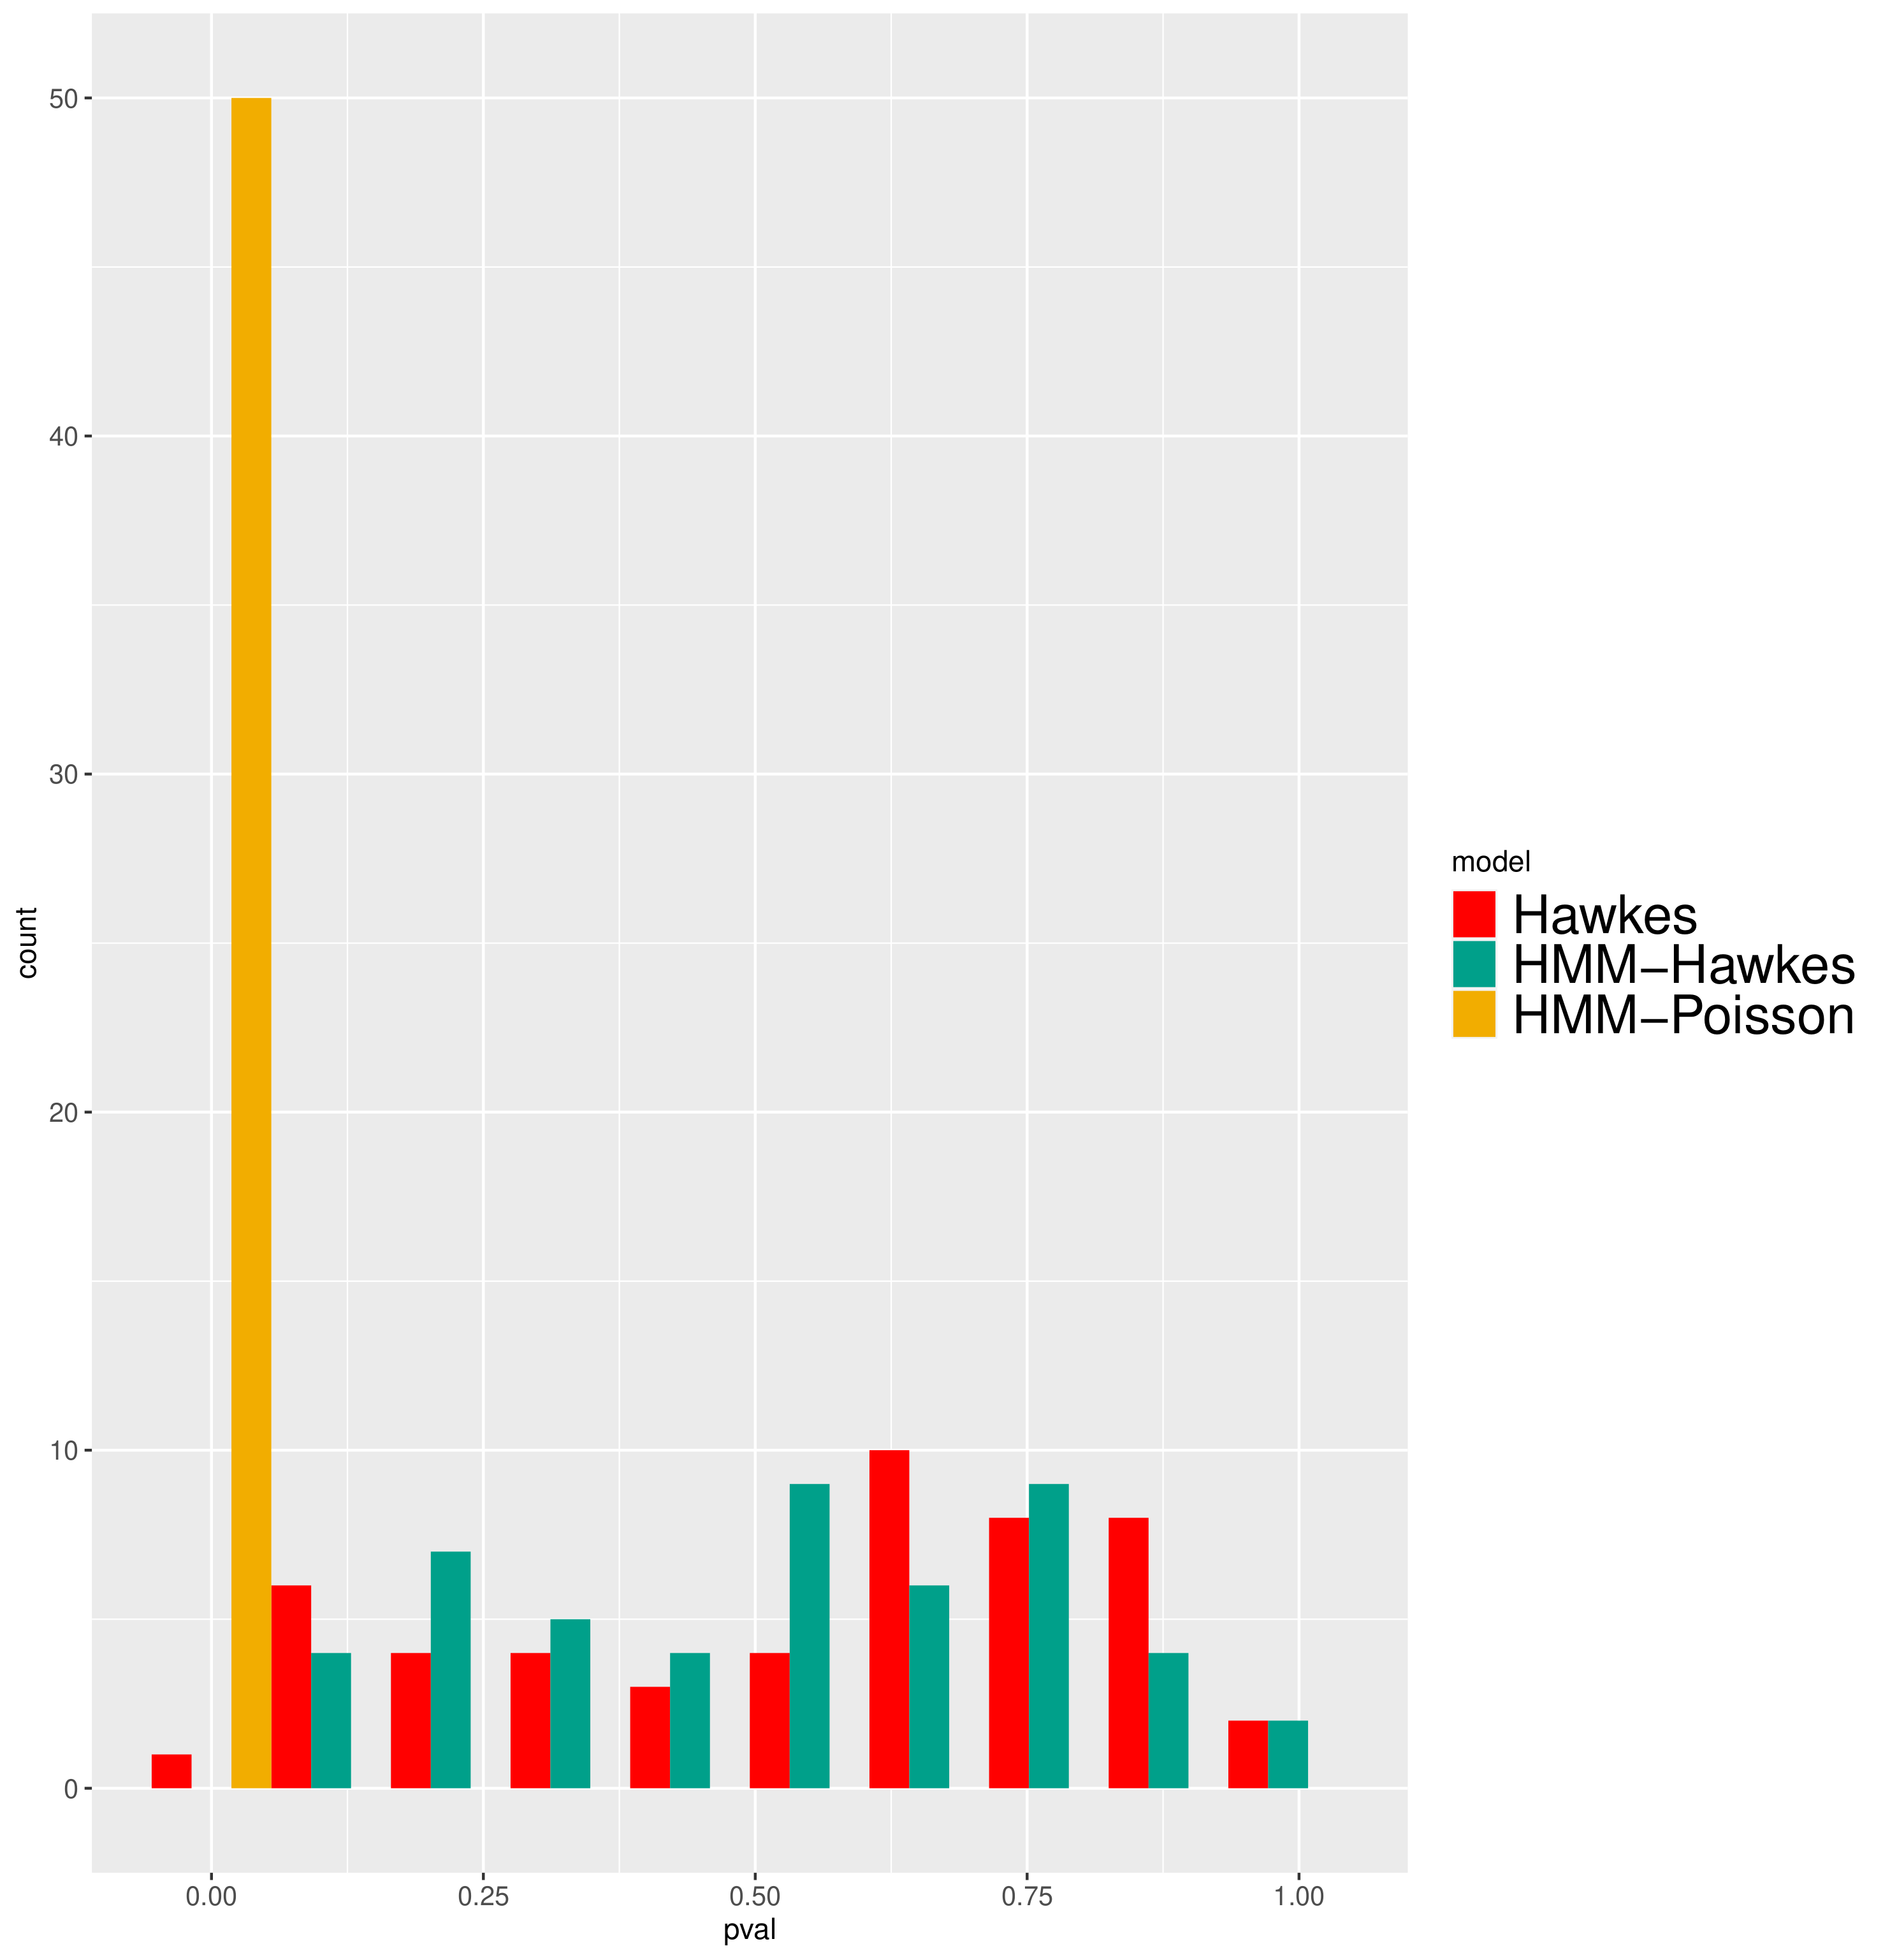
\includegraphics[width=.4\textwidth]{\figcp/Bon24-GOF-Ex1-Pval}
      \end{tabular}
    \end{tabular}
  \end{center}
  
  \bigskip \bigskip 
  \begin{itemize}
    \item The test rejects the homogeneous Poisson but does not differentiate the homogeneous Hawkes process from the HMM-Hawkes process.
  \end{itemize}

}

%====================================================================
\frame{\frametitle{Synthetic data: Goodness-of-fit (2/2)}

  \begin{center}
    \begin{tabular}{cc}
      \begin{tabular}{p{.45\textwidth}}
      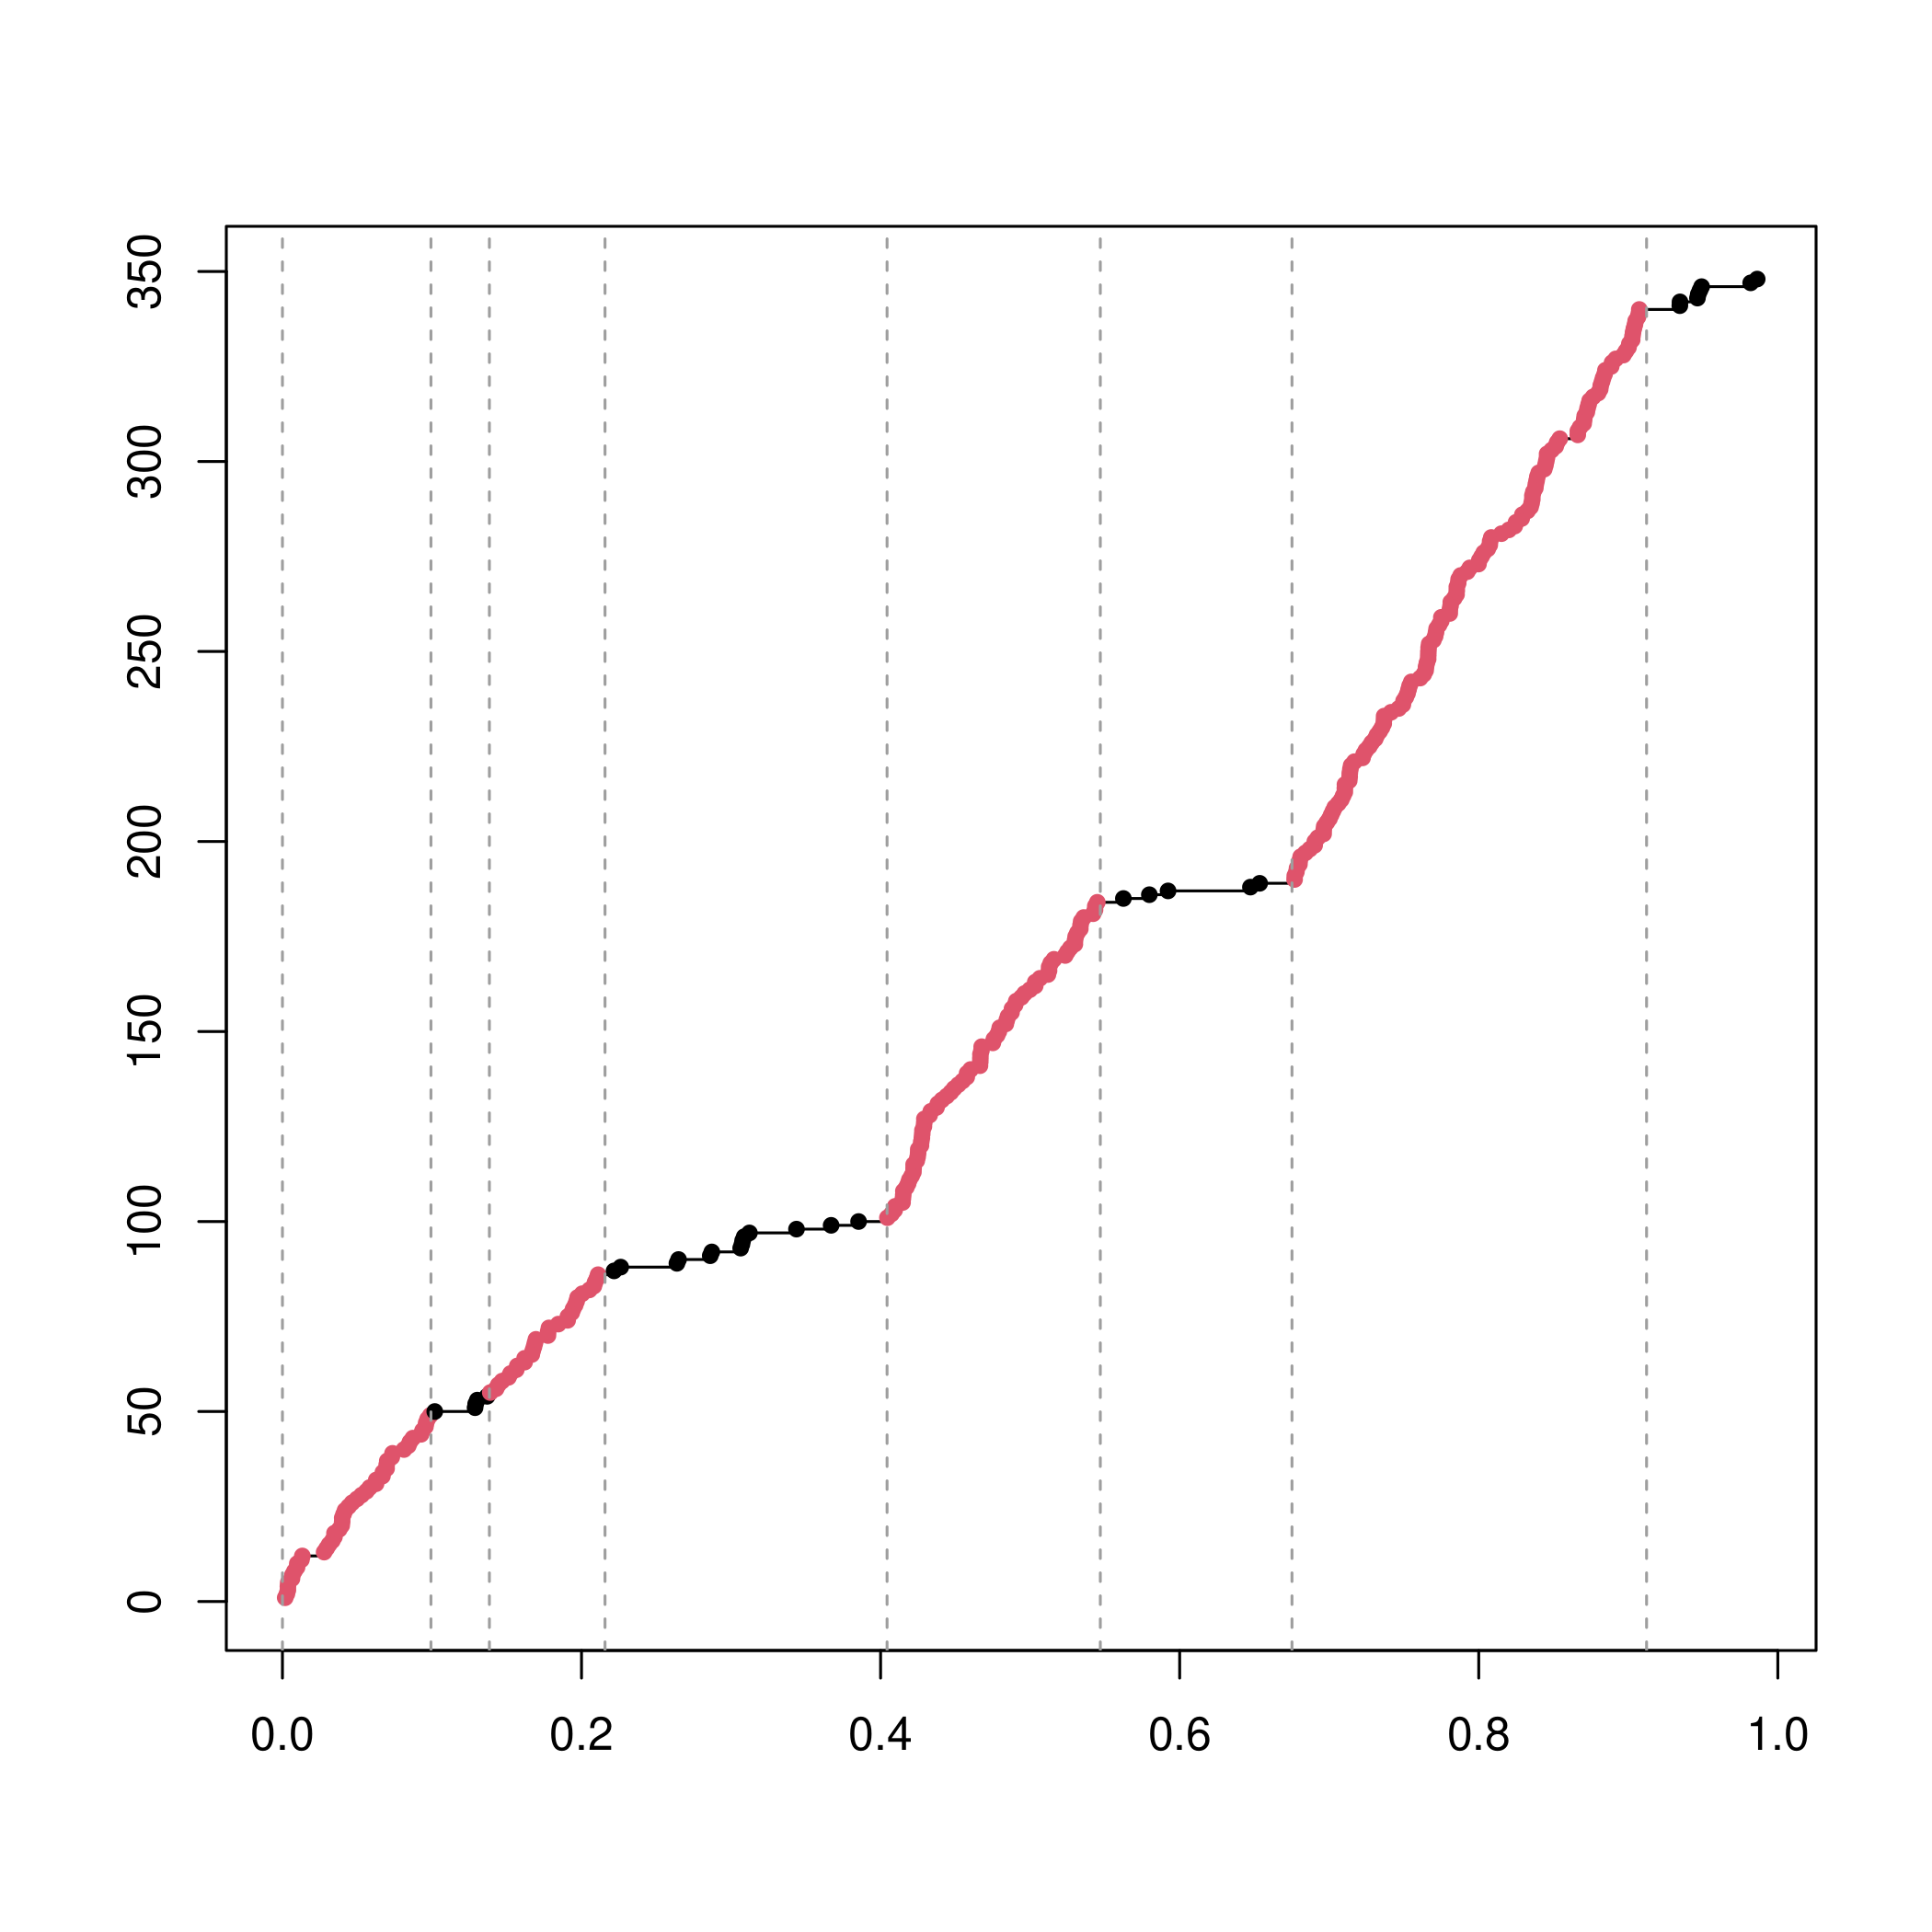
\includegraphics[width=.4\textwidth]{\figcp/Bon24-GOF-Ex2-Path}
      \end{tabular}
      &
      \vspace{-.05\textwidth}
      \begin{tabular}{p{.45\textwidth}}
      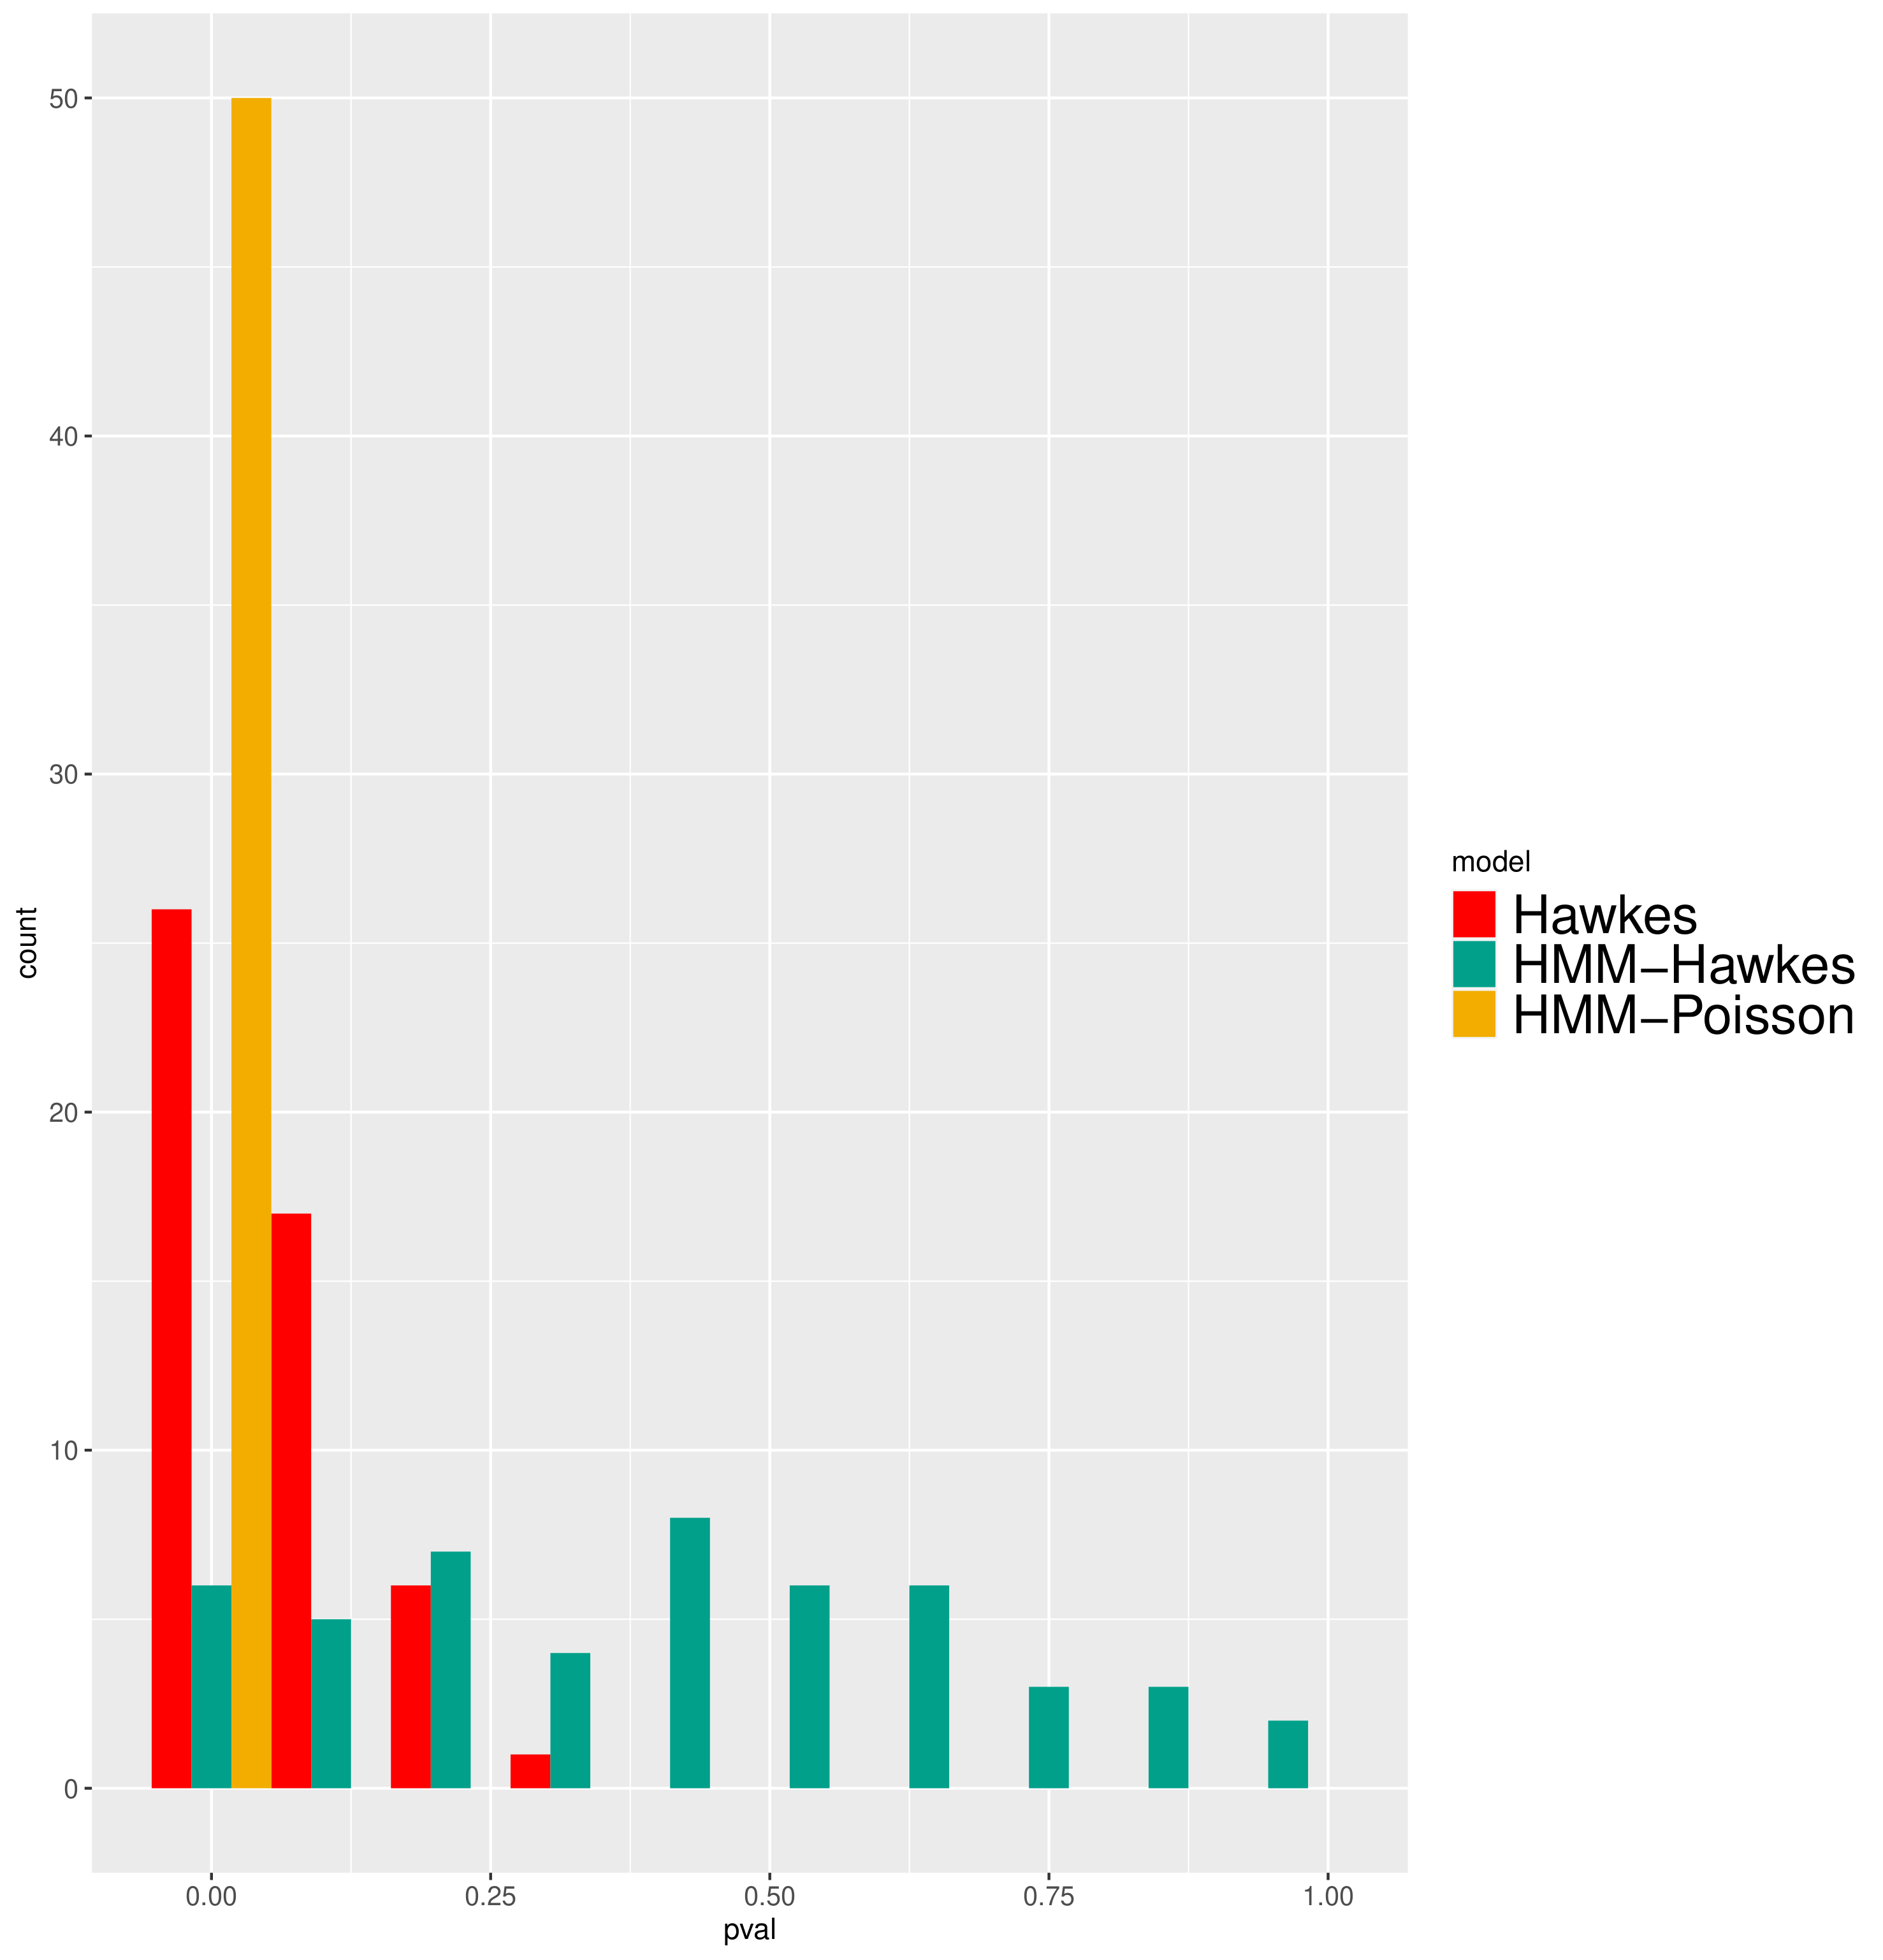
\includegraphics[width=.4\textwidth]{\figcp/Bon24-GOF-Ex2-Pval}
      \end{tabular}
    \end{tabular}
  \end{center}
  
  \bigskip \bigskip 
  \begin{itemize}
    \item The test is able to detect that the point process is neither an homogeneous Hawkes nor a HMM-Poisson process
  \end{itemize}

}

%====================================================================
\frame{\frametitle{Bat cries} 
  
  Recording of bat cries over one night:
%   $$
%   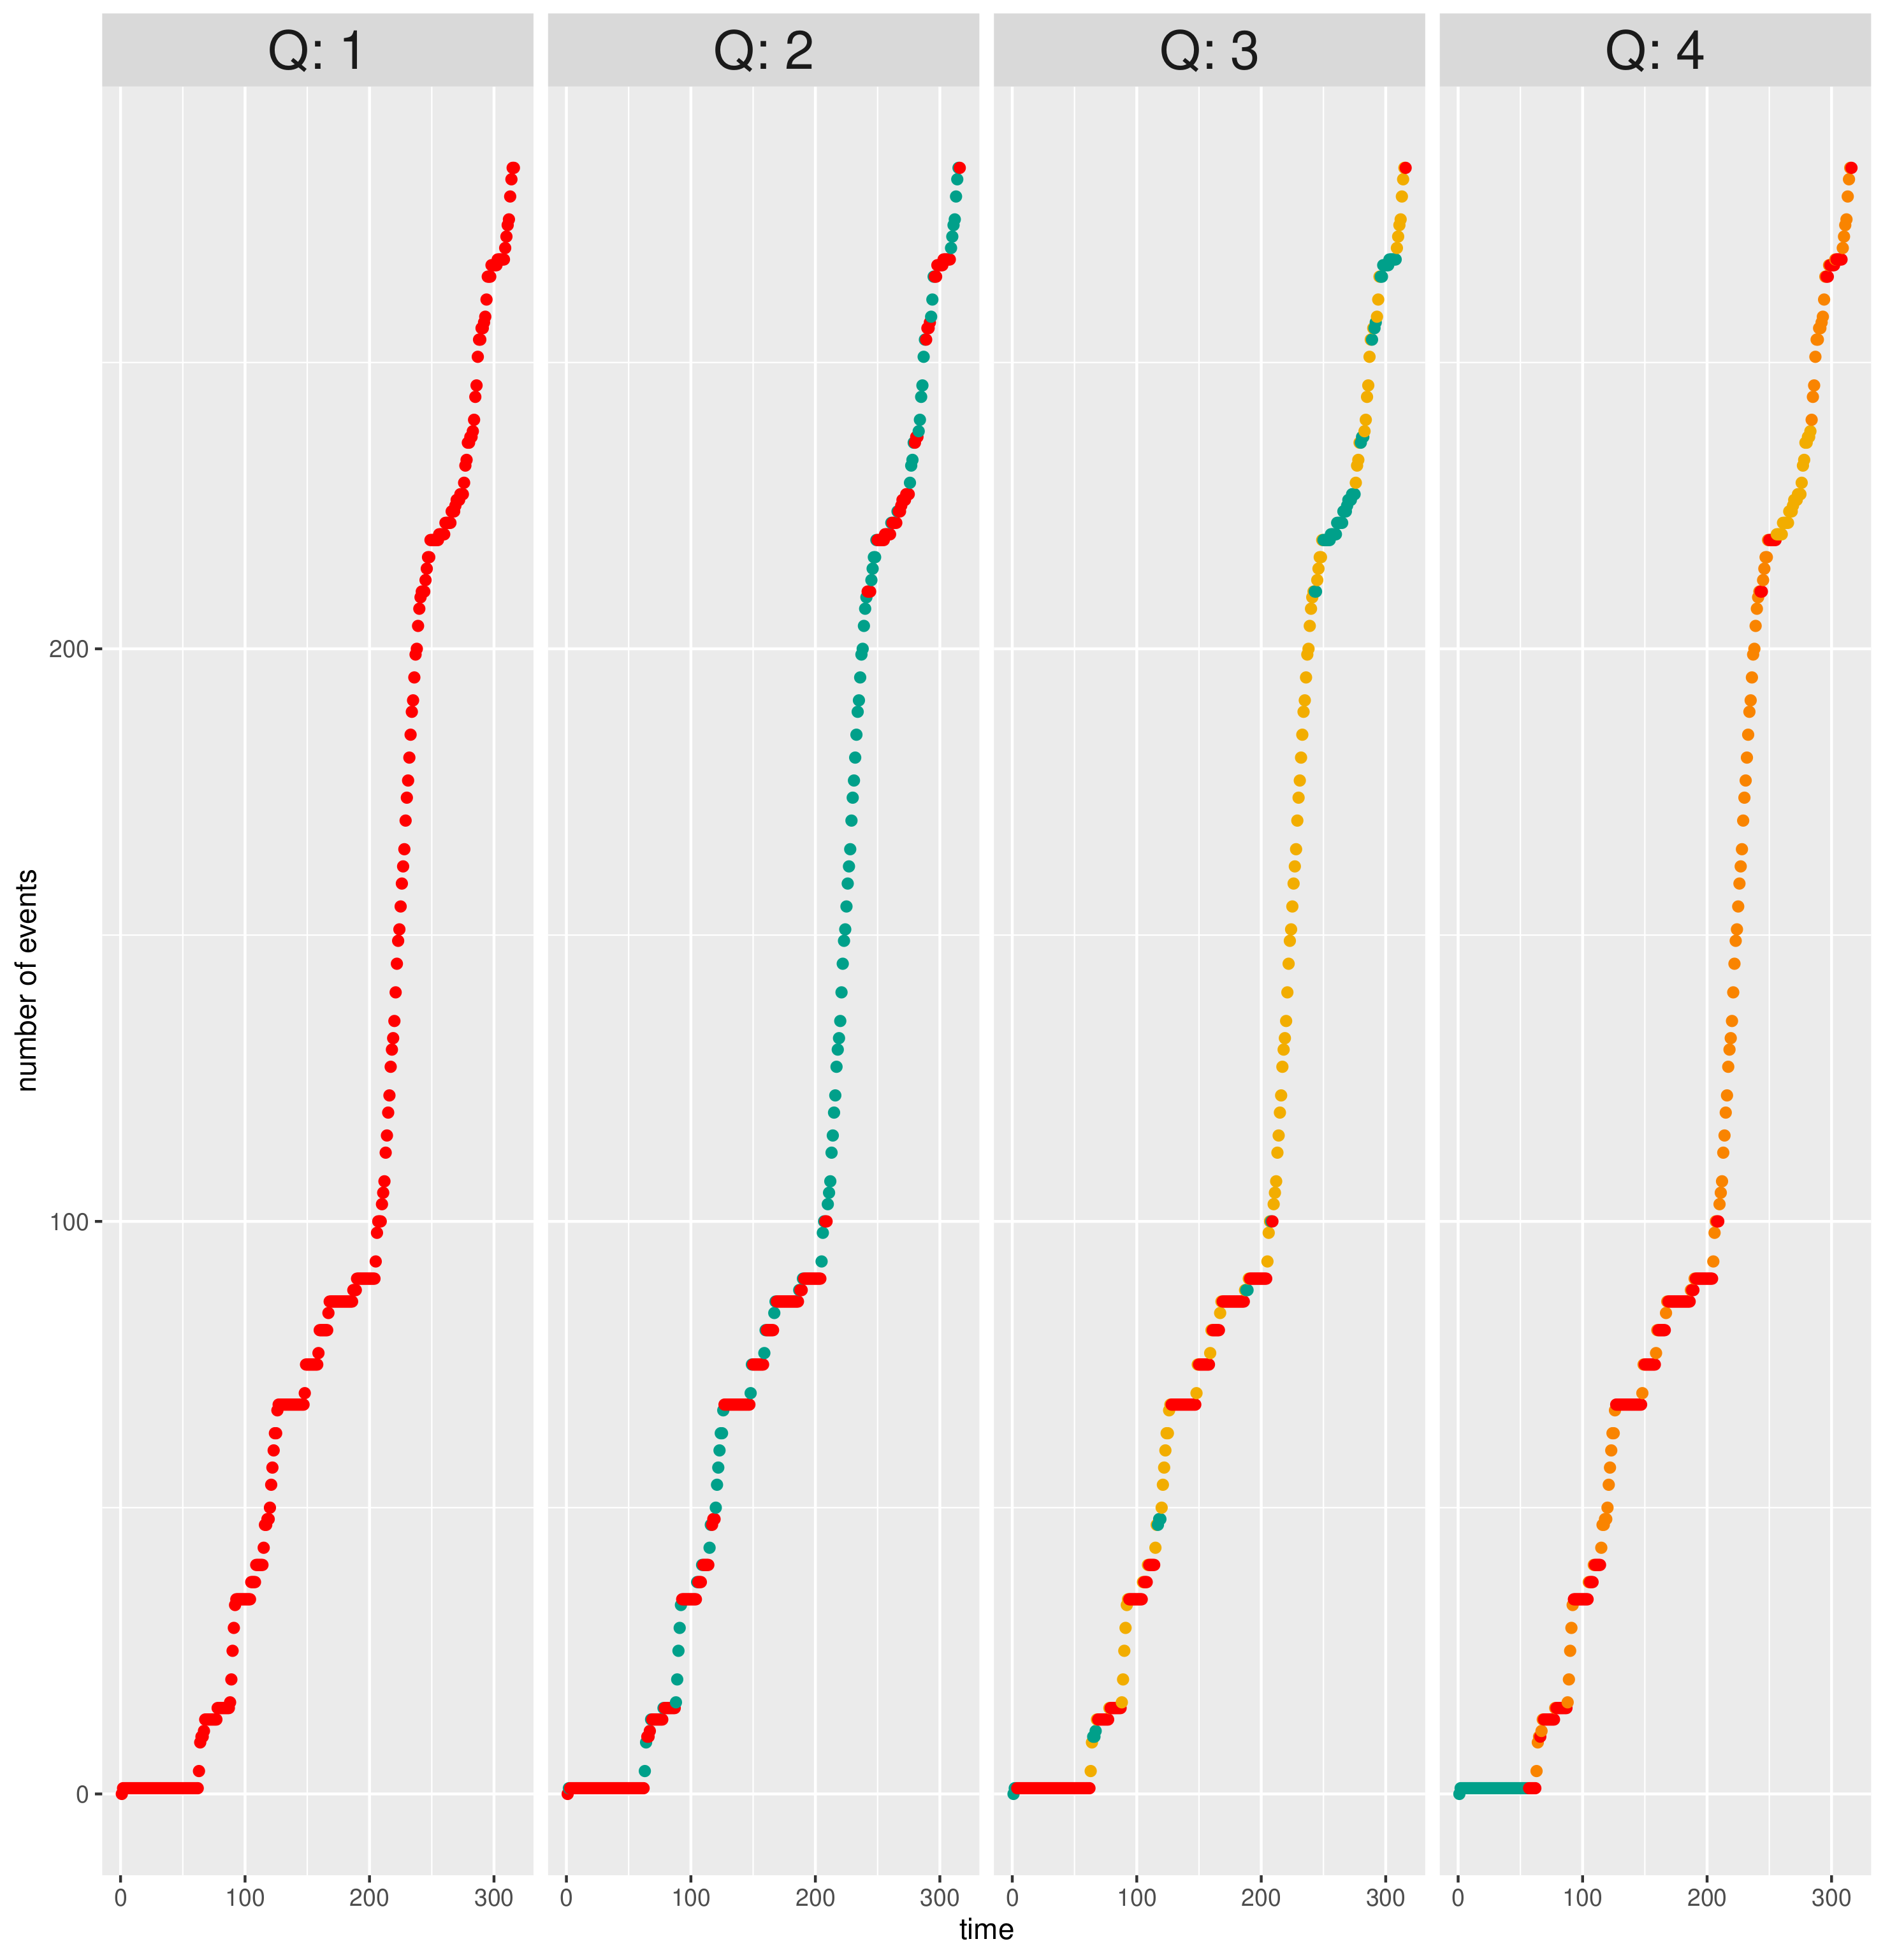
\includegraphics[width=.9\textwidth, height=.5\textwidth]{\figcp/Bon24-Hawkes-CompareQ}
%   $$
  $$
  \begin{tabular}{cccc}
    $Q = 1$ & $Q = 2$ & $Q = 3$ & $Q = 4$ \\
    \includegraphics[width=.2\textwidth, height=.4\textheight, trim=20 20 20 20, clip=]{\figchiro/Chiro-seq99} &
    \includegraphics[width=.2\textwidth, height=.4\textheight, trim=20 20 20 20, clip=]{\figchiro/Chiro-seq99-N692-Qmax5-Q2tau} &
    \includegraphics[width=.2\textwidth, height=.4\textheight, trim=20 20 20 20, clip=]{\figchiro/Chiro-seq99-N692-Qmax5-Q3tau} &
    \includegraphics[width=.2\textwidth, height=.4\textheight, trim=20 20 20 20, clip=]{\figchiro/Chiro-seq99-N692-Qmax5-Q4tau} 
  \end{tabular}
  $$
  \begin{itemize}
    \item $Q = 2, 3, $ hidden states?
    \item States = behavior (transit, foraging), species?
  \end{itemize}


}

%====================================================================
%====================================================================
\section*{Future works}
\frame{\frametitle{Outline} \tableofcontents[currentsection]}
%====================================================================
\frame{\frametitle{Some future works (1/2)} 

  \paragraph{Multivariate Hawkes process:} Consider $p$ simultaneous processes $(N^{(i)})_{1 \leq i \leq p}$ (neurons, bat species, ...)
  $$ 
  \lambda^{(i)}(t)=  \lambda_{0}^i + \underset{i=1}{\overset{M}{\sum}} \underset{T_k^j  < t}{\sum} h_{i,j}(t-T_k^j) 
  $$    
  
  \bigskip
  {Exponential version:} 
  $$
  h_{i,j}(t-T_k^j) = a_{i, j} e^{-b (t - T_k^j)}
  $$
  where sparse interaction matrix $A = [a_{i, j}]_{1 \leq i, j \leq p}$
  
  \begin{tabular}{ll}
    \hspace{-.04\textwidth}
    \begin{tabular}{p{.5\textwidth}}
      \begin{itemize}
        \item Interaction network between neurons, species, ...
      \end{itemize}
    \end{tabular}  
     &
    \hspace{-.04\textwidth}
    \begin{tabular}{l}
      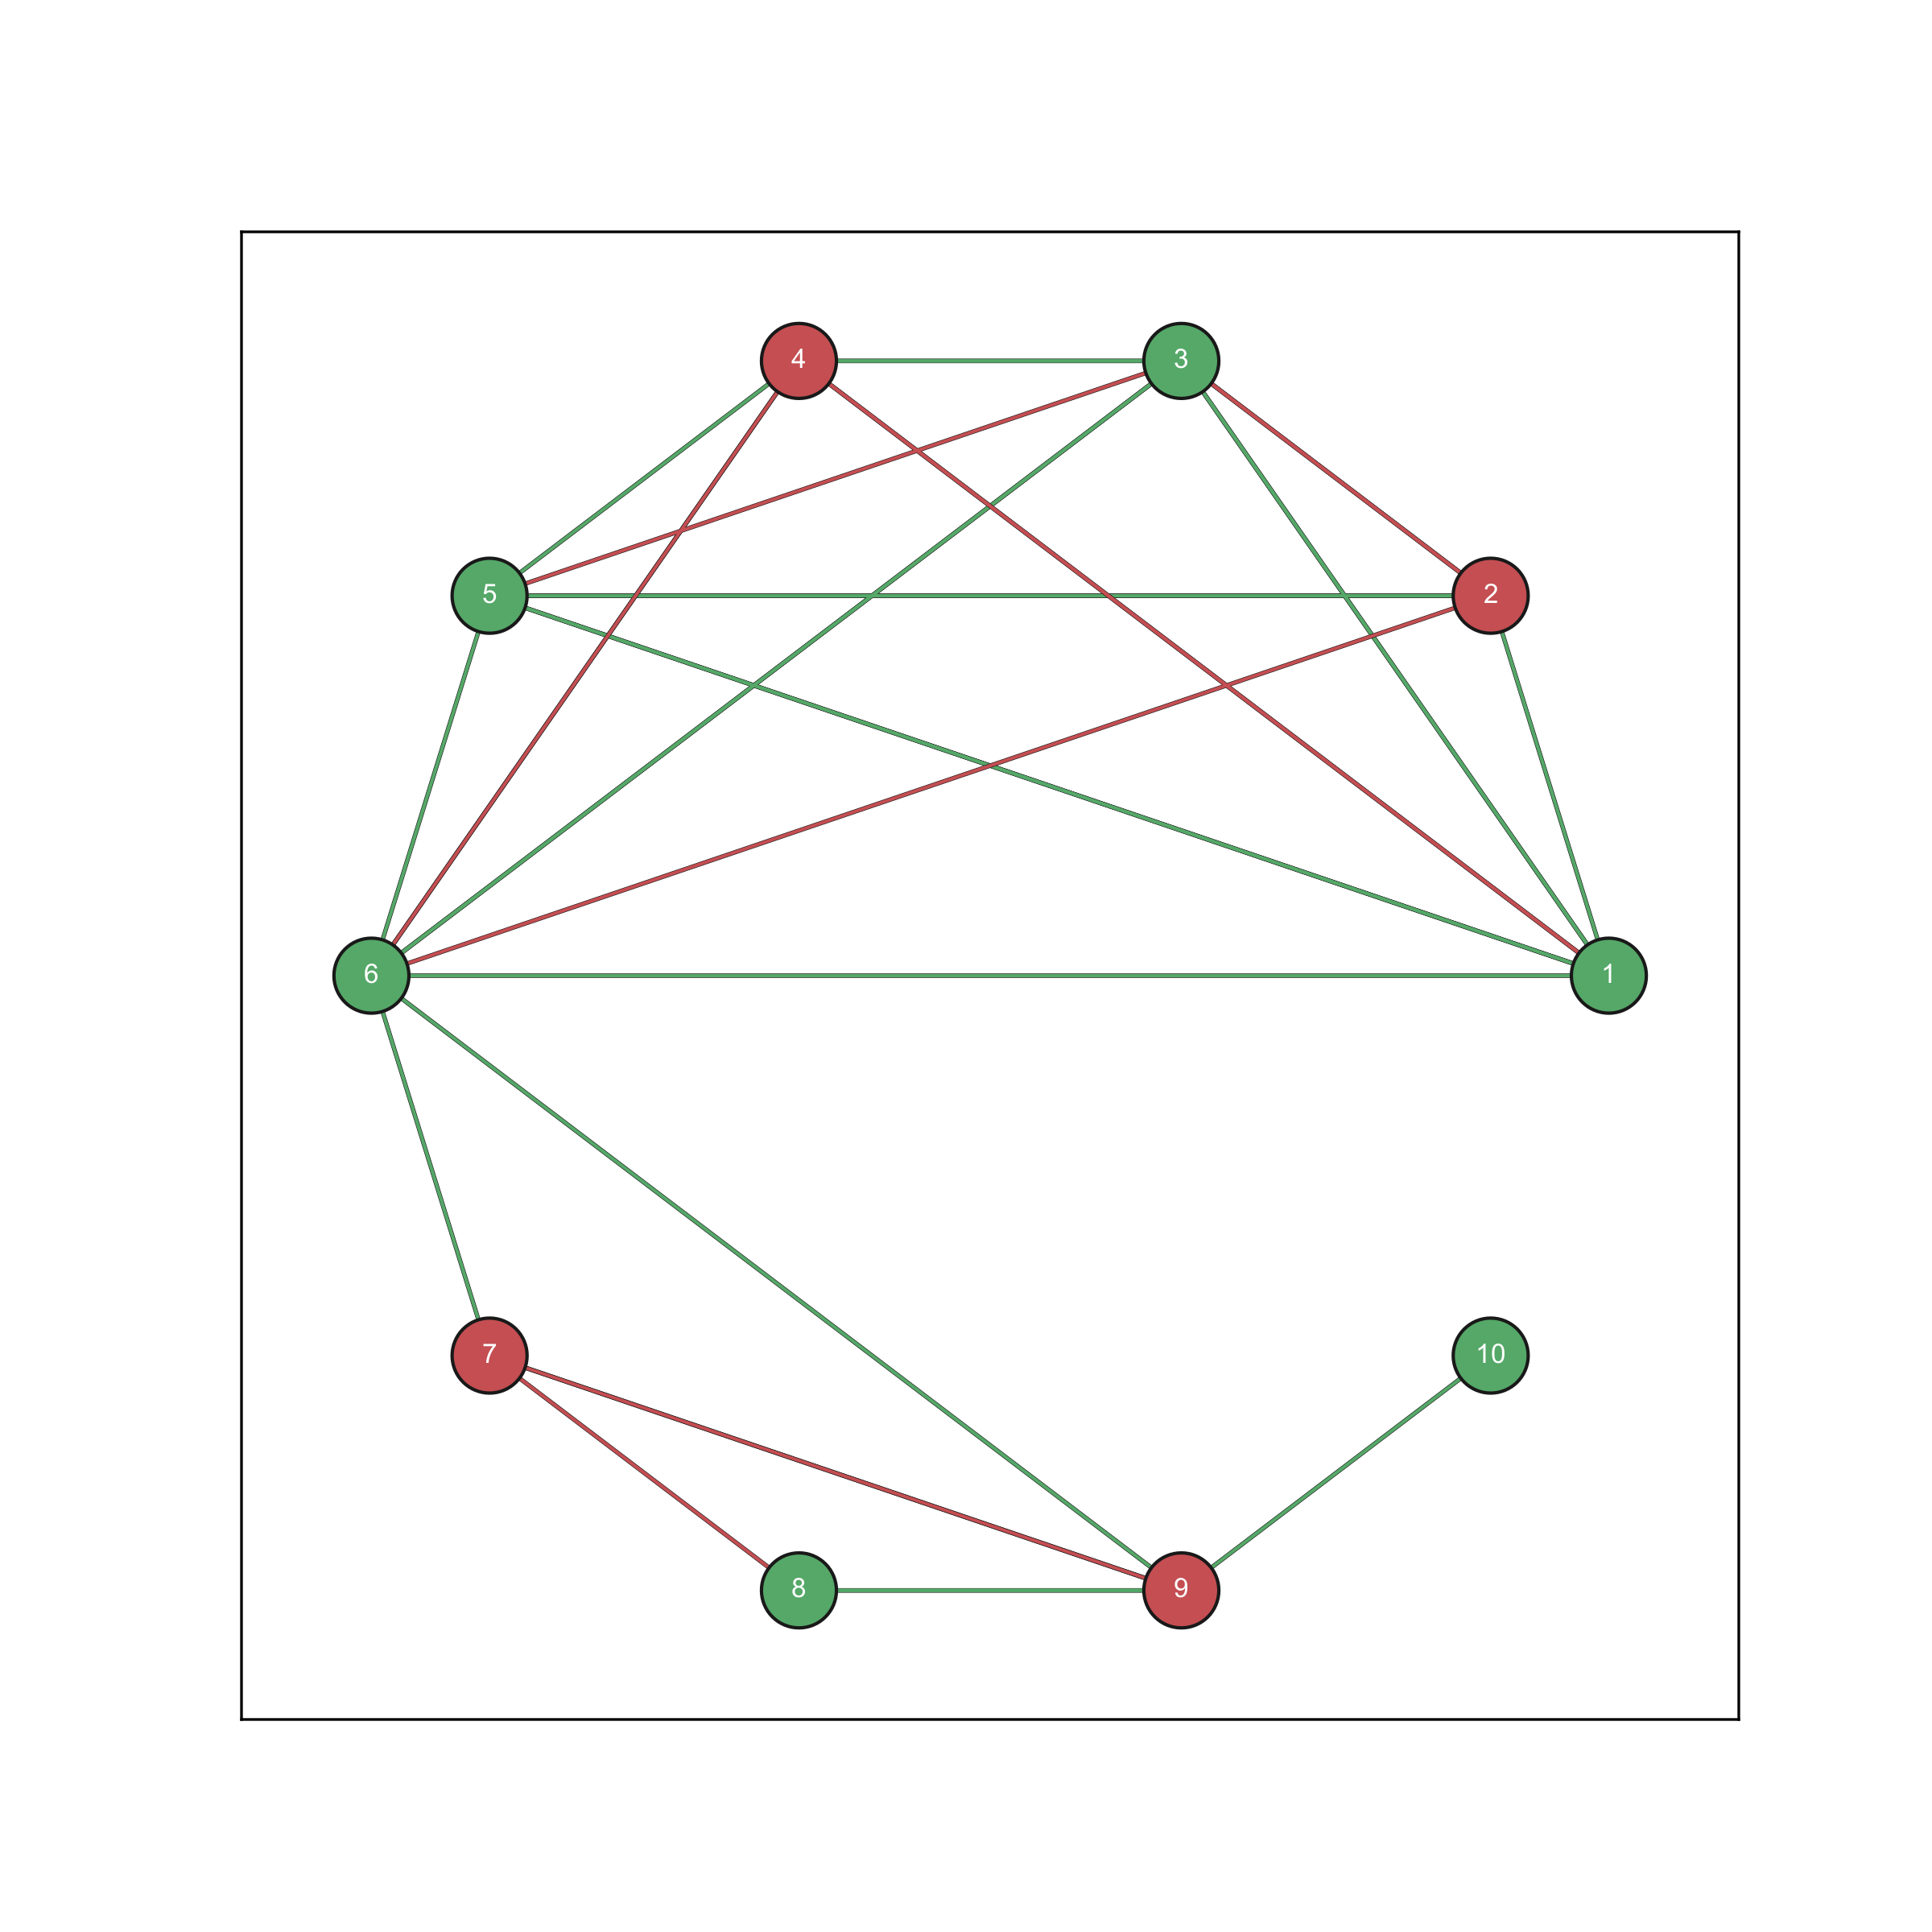
\includegraphics[width=.3\textwidth]{\figcp/Bon24-Network}
    \end{tabular}  
  \end{tabular}  

}

%====================================================================
\frame{\frametitle{Some future works (2/2)} 

  \paragraph{Modelling inhibition:} Non-linear Hawkes process 
  $$ 
  \lambda(t)= \phi \left( \lambda_0 +  \underset{T_k \leq t}{\sum} h(t-T_k) \right)
  $$  

  \bigskip \bigskip \pause
  \paragraph{Effect of the hidden state:} State-dependent parameters $\alpha$ and/or $\beta$
  $$
  Y_k \mid \{Y_\ell\}_{\ell \leq k-1} 
    \sim \mathcal{P}\left(\emphase{\mu_{Z_k}} + \sum_{\ell = 1}^{\infty} \emphase{\alpha_{Z_k}} (\emphase{\beta_{Z_k}})^\ell Y_{k-\ell} \right)
  $$  

}

%====================================================================
\frame{ \frametitle{References}
  {
   \footnotesize
   \bibliography{/home/robin/Biblio/BibGene}
   \bibliographystyle{alpha}
  }
}

%====================================================================
%====================================================================
\backupbegin 
\section*{Backup}
%====================================================================
\frame{ \frametitle{Backup}

  \paragraph{Conversion formulas} from continuous to discrete Hawkes
  $$
  \alpha  = \frac{e^{b \Delta} - 1}{b}, \qquad \beta = e^{-b \Delta}
  $$
    
  \bigskip \pause 
  \paragraph{3-step initialization}
  \begin{itemize}
    \item Homogeneous Hawkes for the reproduction parameters $\alpha$ and $\beta$ \\
    ({\tt hawkesbow} R package \refer{Che21})
    \item Poisson-HMM for the rates $\mu_1, \dots, \mu_Q$
    \item Correction $\mu_k \rightarrow \widetilde{\mu}_k$ to account for reproduction rate
  \end{itemize}
  
}

%====================================================================
\backupend 

%====================================================================
%====================================================================
\end{document}
%====================================================================
%====================================================================
  
  \begin{tabular}{cc}
    \hspace{-.04\textwidth}
    \begin{tabular}{p{.5\textwidth}}
    \end{tabular}
    & 
    \hspace{-.02\textwidth}
    \begin{tabular}{p{.5\textwidth}}
    \end{tabular}
  \end{tabular}


